\documentclass[11pt,a4paper,twoside,twocolumn]{article}

\usepackage{graphicx,parskip,times,amsfonts,amsmath}
%\usepackage{url}
%\usepackage{html}
\usepackage{esc-handbook-org}
\usepackage{eurosym}
%\usepackage{chapterbib}
\usepackage{natbib}
\usepackage{a4,a4wide}
\usepackage[english]{babel}
\usepackage{amssymb,amsmath,amsfonts}
\usepackage{bibunits}


%%/Users/Dierk/IUB documents 2005/Research Reports/Research Report 2005/SinDynamics.pdf
\hyphenation{Schlei-cher} \hyphenation{geo-me-try}
\newcommand{\C}{\mathbb{C}}
\newcommand{\R}{\mathbb{R}}
\usepackage{latexsym}
\newcommand{\bbbr}{\mathbb{R}}
\newcommand{\bbbn}{\mathbb {N}}
\newcommand{\bbbc}{\mathbb {C}}

%---------------------PDF-definitions--------------------------------------
\usepackage[pdftex,           %%% hyper-references for pdflatex
  hypertexnames=false,%       %%% needed for correct links to figures
  breaklinks=true,%           %%% break links if exceeding a single line
  colorlinks=true,%           %%% to underline links instead of boxing
  urlcolor=blue]{hyperref}    %%% blue instead of cyan URLS
%---------------------end-of-PDF-definitions-------------------------------


\newcommand{\mycaption}[1]{\caption{{\footnotesize #1}}}
\renewcommand*{\cleardoublepage}{\clearpage\if@twoside \ifodd\c@page\else
    \hbox{}
    \if!\blankpagetext!\else
    \vfil \begin{center} \setlength{\fboxsep}{3mm}%
    \framebox{\blankpagetext}
    \end{center}\vfil\vfil \fi
    \newpage\if@twocolumn\hbox{}\newpage\fi\fi\fi}
\newcommand*{\resetpages}{\cleardoublepage\pagenumbering{arabic}}
\raggedbottom \pagenumbering{Roman}

\setlength{\parskip}{0pt plus 1pt}
\begin{document}
% Robert's hack:
\def\Hchapter{\paragraph}
%
\graphicspath{{./MathTheoPhys/}{./Physics/}{./Nano/}{./LifeSciences/}{./GeoAstro/}{./EECS/}}

\title     {School of Engineering and Science \\
            Research Report 2005} \shorttitle{RP 2006}
\author    {Anke Allner}
\date      {2006 January 18}
\masterfile{SES--RR--2006} \issue     {0} \revision {1} \version
{2}{0}{27.12.05}{Test}

\shorttitle{Table of Contents} \tableofcontents \resetpages
%\shorttitle{Introduction}
\section{Introduction}

With the outstanding financial investment of the Jacobs Foundation
in the Jacobs University on October 31, 2006 the future perspective
of the University and in particular the School of Engineering and
Science is on steady and forseeable grounds. This, and the advent of
the new president Professor Dr. Dr. h.c. mult. Joachim Treusch, who
formally took office by July 1, 2006, eventually resulted in a
reformulation of the key mission and the main research objectives of
the university. The main scientific activities of the School can be
considered to be perfectly consistent with the new objectives.

\subsection{The Mission}

The Jacobs University Bremen has been designed and developed as an
international research university using the anglo-saxon template,
and incorporating the European Bologna Process into its teaching
model. The main mission is to academically educate bright young
people, irrespective of their nationality, religion, sex, race and
financial conditions, in order to prepare them for future leading
roles in our globalized world. Thus, the University is designed to
provide significant contributions towards a peaceful, and
sustainable development of mankind. As a campus university where
students from more than 80 nations live and learn together in
colleges, intercultural understanding and collaboration in daily
life is trained as a byproduct of the university education.

\null
 Research and teaching are pursued on the same level and take
into account the requirements of practical life in enterprises and
industry. Interdiciplinarity constitutes the key concept. Research
at the Jacobs University Bremen aims at delivering key contributions
towards the main challenges of mankind, namely \\

\begin{myitemize}
\item   energy and materials,
\item  water and food,
\item   health,
\item "Bildung" and communication,
\item peace and conflict management.
\end{myitemize}


\null
 The School of Engineering and Science contributes with its
activities mainly towards the former three of these, although its
strong electrical engineering faculty addresses technological issues
that are closely related to the latter two.

The scientific objectives of Jacobs University concentrate in five
broad areas, namely \\

\begin{myitemize}
\item bio-geo-marine resources - from molecules towards technologies
\item  modelling of complex systems - computer simulation, visualisation, networks and management
\item changing societies, cultures, and institutions -  aspects of globalisation
\item   Asia and Europe - historical,
psychological and cultural perspectives
\item productive adult development \item "Bildung" and work
\end{myitemize}


\null
 The five research fields of the School of Engineering and
Science that have been emerging during the founding years contribute
towards the first two of these: Projects within "Information and
Communication Technologies" are directly related to the second
research area. Topics addressed by our "Life Sciences" and
"Geosciences and Astrophysics"  contribute to the first as well as
to the second area. "Nanoscience and Material Research" and
"Mathematics and Theoretical Physics" establish the scientific
backbones of the above. These provide important scientific tools and
the key methods for successfully tackling questions at the
interfaces between the conventional disciplines.

\null
The latter, namely science across disciplinary boarders is
indeed the outstanding - if not the main - trademark of research and
development,  and teaching at the  School of Engineering and
Science.


\subsection{Factual Development During the Founding Period}

\subsubsection{Students}
During the course of the past founding years, the School of
Engineering and Science has been showing remarkable growth, in
quantity as well as in quality. The number of undergraduate
students, starting in 2001 with 67 has now reached its preliminary
saturation at 381 students (Fig.~\ref{fig:students}). Basically this
is dictated by the number of college places and the fact that
according to planning 2/3 of the total number of students can be
admitted to programs of the School. There are now 12 undergraduate
programs of which 10 are formally accredited.


In 2004, for the first time a significant number (48) of graduate
students were admitted to the graduate programs of the School. Since
then, the number of graduate students has been growing to an
impressive total of 223 out of which 142 are PHD-students
(Fig.~\ref{fig:students}). By now, the school has successfully
established 7 graduate programs on the master's level.

\begin{figure}[ht]
  \begin{center}
   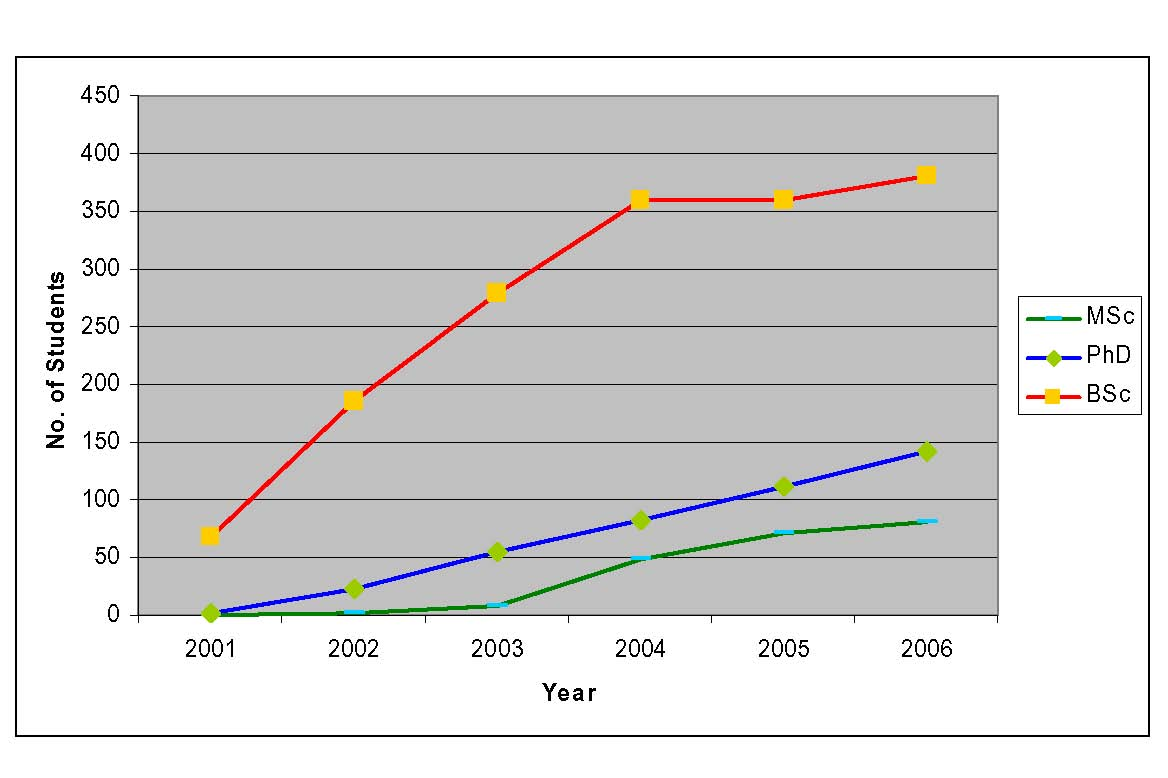
\includegraphics[width=\hsize]{Students.jpg}
   \end{center}
\caption{Temporal Development of Number of Students in the School of
Engineering and Science \label{fig:students}}
\end{figure}

\label{students}

\subsubsection{Publications}

During the founding period, the scientific output of the School,
measured in terms of the number of publications, has been growing
from initially 144 to 389 in 2006, after an intermediate decrease in
2004 which can be understood by having in mind that 2004 has been
the year during which the main research laboratories have been
planned and constructed (Fig.~\ref{fig:publications}). The last of
the laboratories (the EON laboratory) has been finished in 2005.

\begin{figure}[ht]
  \begin{center}
   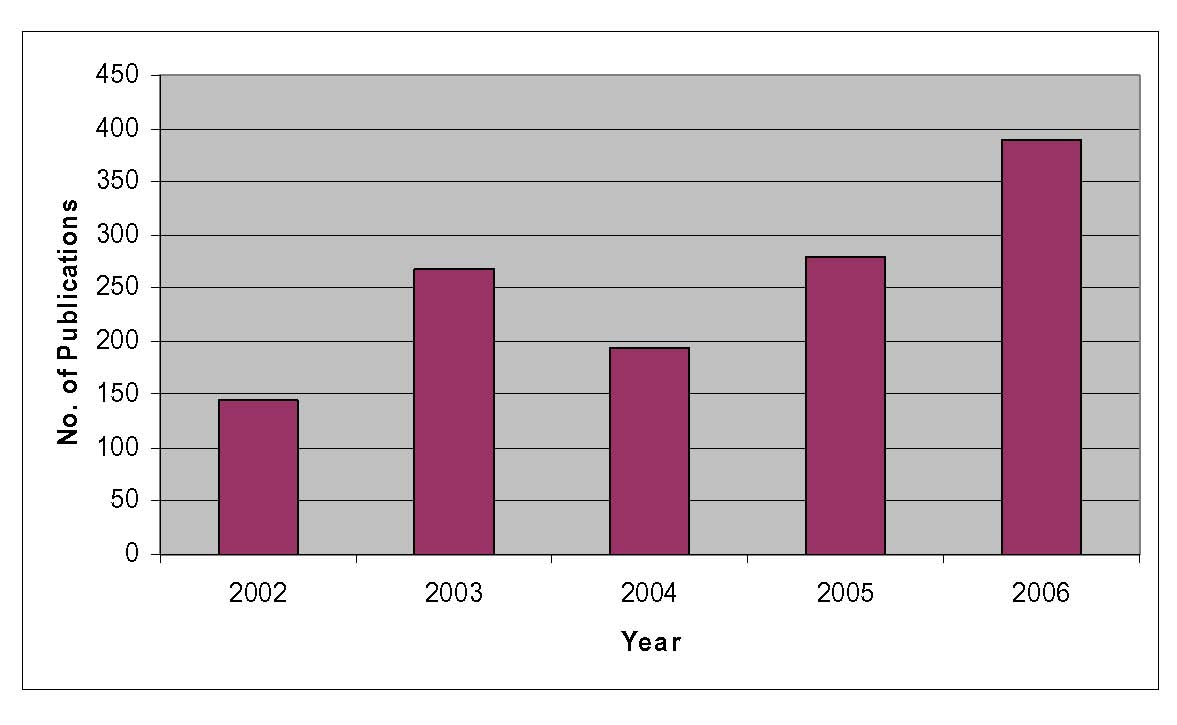
\includegraphics[width=\hsize]{Publications.jpg}
   \end{center}
 \caption{Number of Peer-reviewed Articles, Conference Proceedings, Articles in Encycl./Handbooks,
 Monographs/Books, Editor-ship, and Contribution in Ed. Volumes
 \label{fig:publications}}
\end{figure}


\subsubsection{Grants}
The development of third party funding is summarized in Figures
\ref{fig:grants1}, \ref{fig:grants2}. Revenues from Research grants
have reached a total of more than 4.000.000 EURO in 2006 which
implies an average revenue per professor of 82.000 EURO.

\begin{figure}[ht]
  \begin{center}
   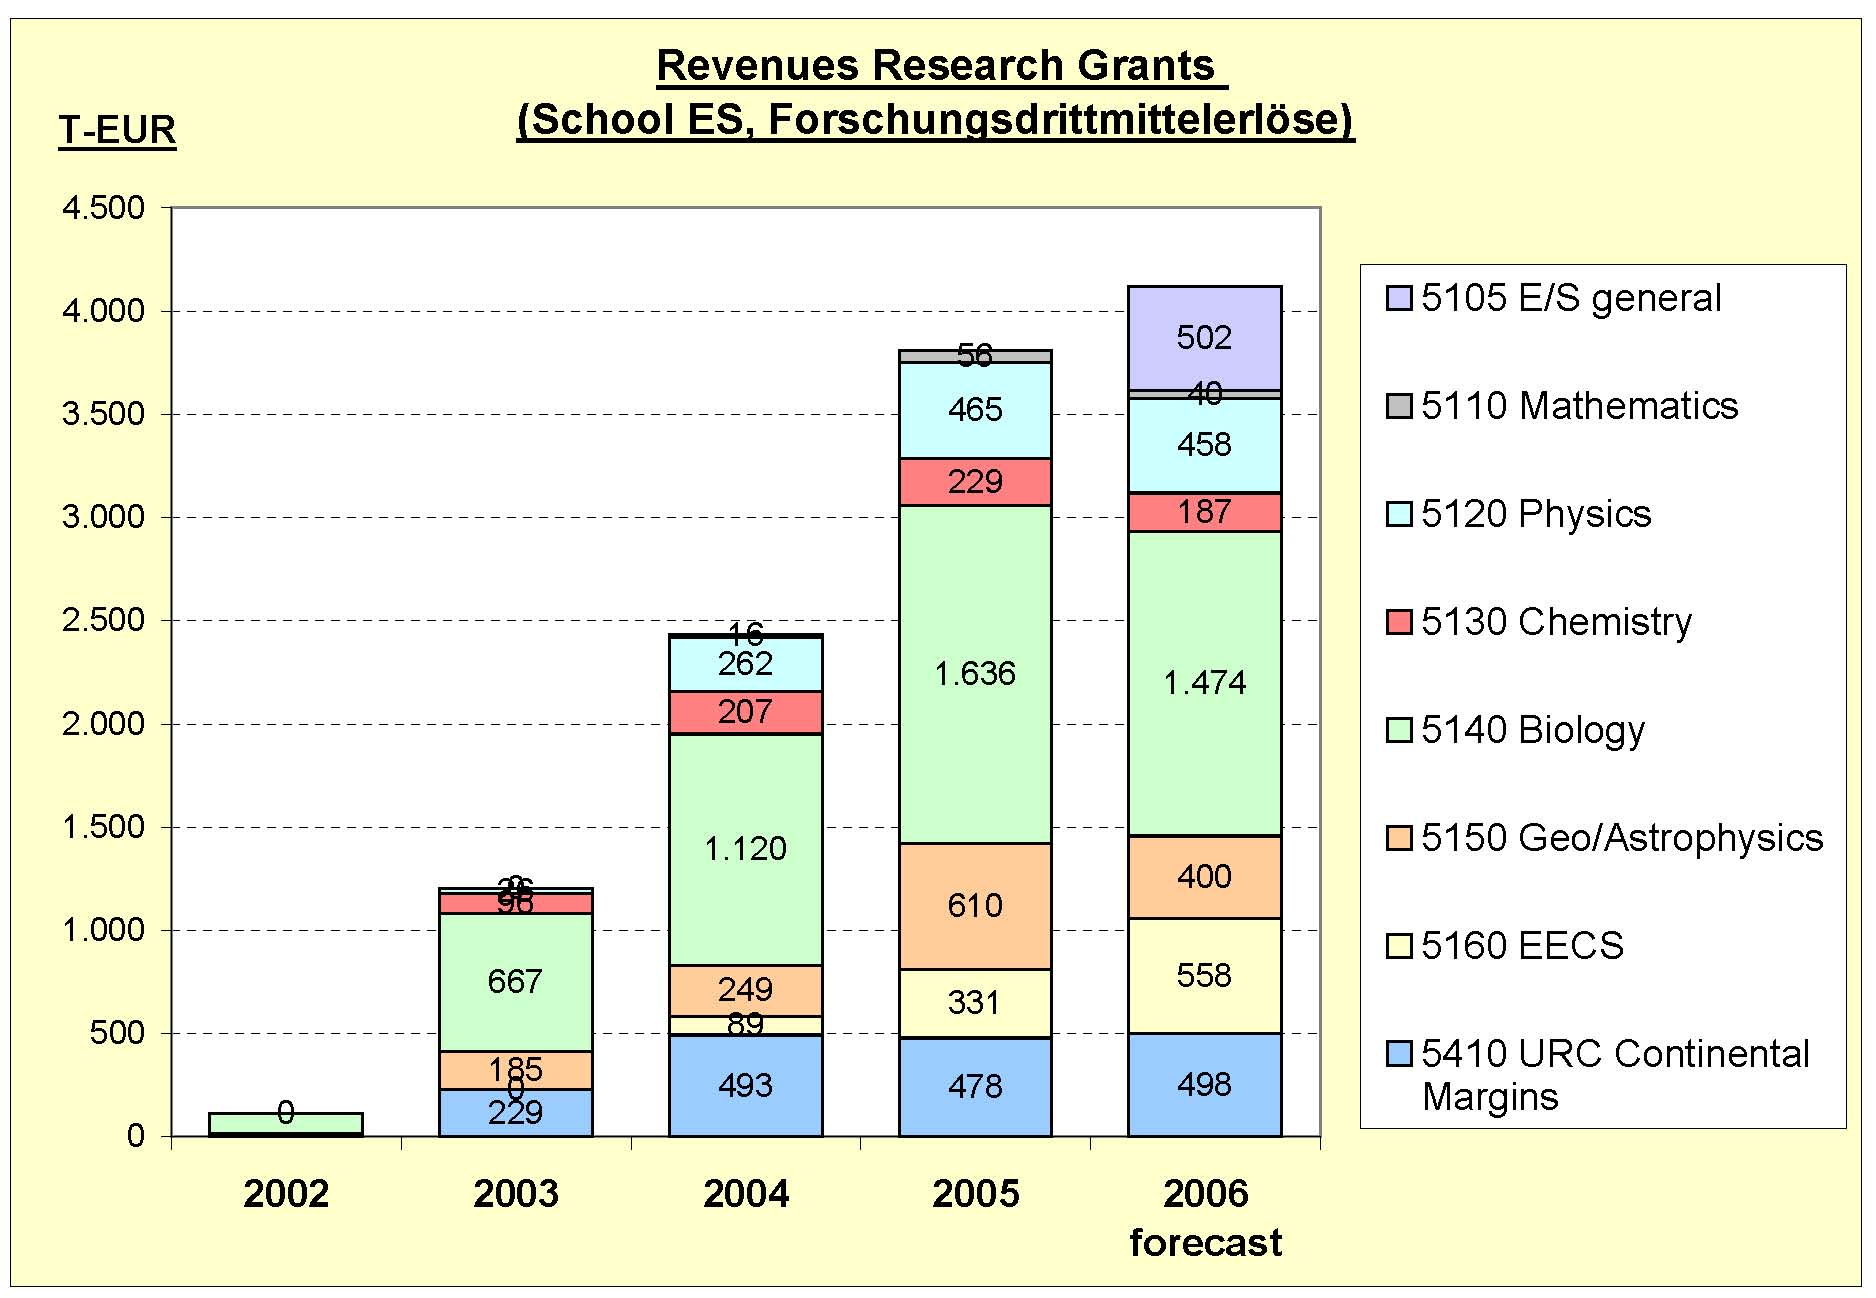
\includegraphics[width=\hsize]{SchoolESGrants-Charts1.jpg}

   \end{center}
 \caption{Research Grants  Revenue
 \label{fig:grants1}}
\end{figure}

\begin{figure}[ht]
  \begin{center}
   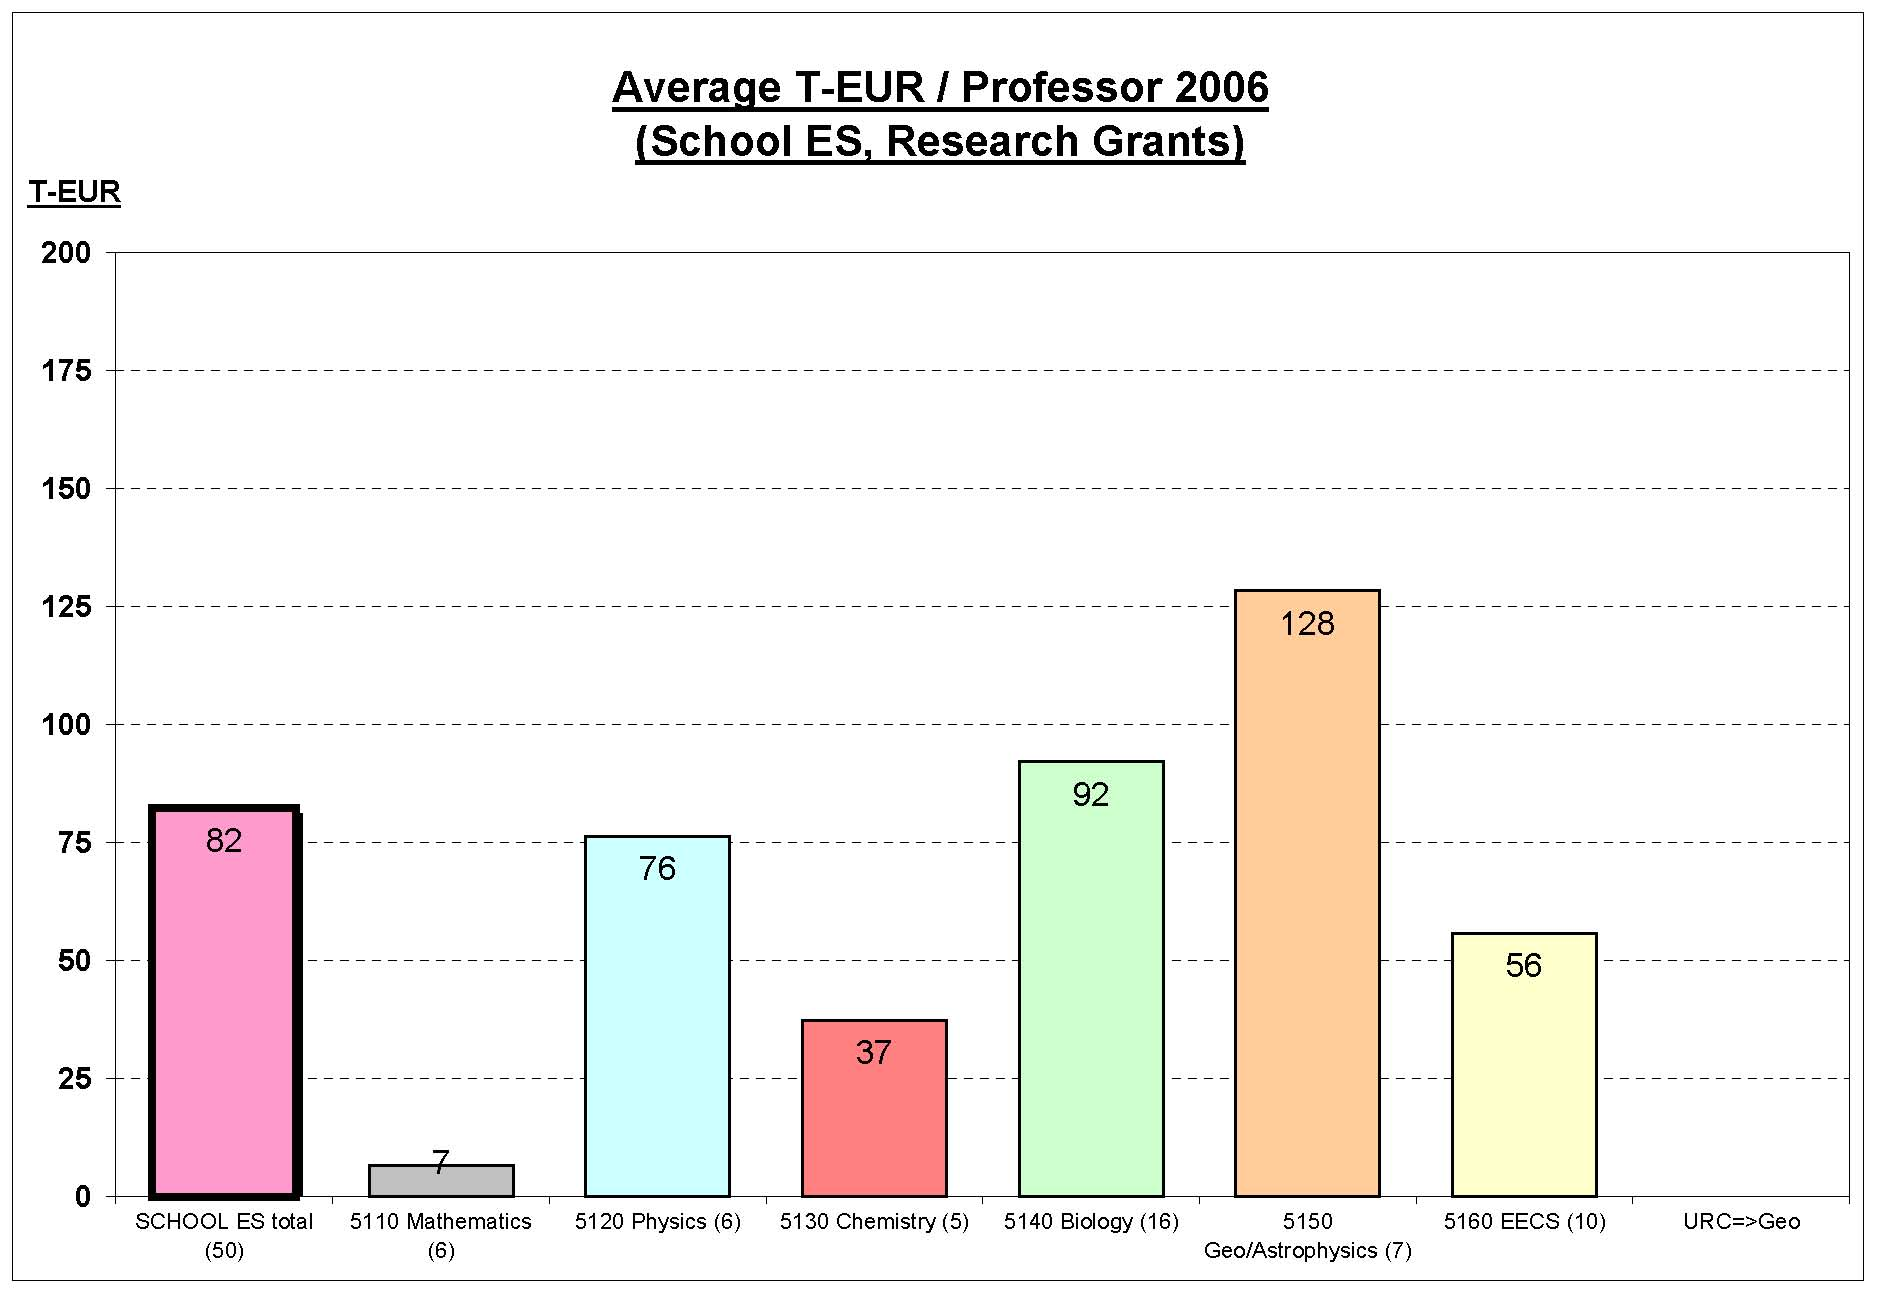
\includegraphics[width=\hsize]{SchoolESGrants-Charts2.jpg}
   \end{center}
 \caption{Research Grants Average T-EUR/Professor
 \label{fig:grants2}}
\end{figure}

\subsection{Personnel 2006} Presently, the school comprises in
total 64 professors out which 4 are adjunct professors, located at
the Alfred-Wegner-Institut in Bremerhaven and the Max-Planck-Insitut
f�r Marine Mikrobiologie in Bremen. Two distinguished professors and
6 university lecturers complete the faculty. In addition, 70
research associates, 5 research assistants, 26 technicians, 1
director and 7 assistants belong to the staff. In 2006, several new
faculty members have been hired.

\begin{myitemize}
 \item   Dr. Ulrich Kleinkath\"ofer, Associate Professor of
Theoretical Physics \item  Jon Wallace, PhD, Assistant Professor of
Electrical Engineering \item  Dr. Lars Linsen,  Associate Professor
of Computational Science and Computer Science \item   Dr. Bendick
Malehko, University Lecturer in Computer Science.
\end{myitemize}

In Mathematics, the visiting professors Prof. G. Litvinov and Prof.
Vladimir Tikhomirov, and Dr. Marc Comerford (research instructor)
left. They are replaced by \begin{myitemize} \item  Dr. Stefan Baier
(Visiting Lecturer for Mathematics) \item Kaivan Mallahi-Karai (PhD,
Visiting Lecturer for Mathematics) \item Dr. Alexei Belov (Visiting
Professor for Mathematics).
\end{myitemize}

The following members of the faculty have been promoted during 2006.
\begin{myitemize}
\item  Dr. Klaudia Brix from Associate to Full Professor
\item Dr. Albert Jeltsch from Associate to Full Professor
\item   Dr. Laurenz Thomsen from Associate to Full Professor
\item Marcus Br\"uggen Assistant to Associate
\item Claus C. Hilgetag, PhD from Assistant to Associate
\item Dr. Ulrich Schwaneberg from Assistant to Associate
\end{myitemize}

\null
Dr. Stefano Carpin, Assistant Professor of Computer Science,
has accepted an offer of an Assistant Professorship at University of
California, Merced, USA, starting on January 1, 2007.

\subsection{International Center for Transdisciplinary Science}
 The "International Center for Transdisciplinary Studies"
has been founded and started to operate. The center invites
internationally highly ranked scientists as fellows for periods of
several weeks, mostly during the summer break. The visiting
scientists are generally expected to participate in ongoing
scientific activities. In 2006, 46 scientists have been
participating, among them 39 from foreign countries:

\null Professor Dr. Roland Benz,   Universit\"at W\"urzburg, Germany
\\
Professor Dr.~Jan Bergstra,  University of Amsterdam, The Netherlands\\
Dr.~Andrey Bessonov, University of Sankt Petersburg, Russia\\
Dr.~S.M. Bezrukov,  National Institute of Health, Bethesda, USA\\
Dr. Georges Bouzerar,   Laboratoire Louis Nel, Grenoble, France\\
Dr. Henk Bruin  University of Surrey, United Kingdom\\
Professor Dr.~Mark Burgess,  University College Oslo, Norway\\
Professor Dr.~Val\'erie Cabuil,     Universit\'e Pierre et Marie
Curie, Paris, France\\
Dr.~Fabio Cavaliere, Universit\'a di Genova, Italy, Professor
Dr.~Shengbo Chen,      Institute of Geography and Natural
Resources, Beijing, China\\
Elizabeth Dan-Cohen,     University of California, Berkeley, USA\\
Professor Dr.~Gero Decher,      Institut Charles Sadron, Strasbourg,
France\\
Dr.~Martin Evans,        University of Edinburgh, United Kingdom\\
Dr.~Tom Fisher,      University of Cambridge, United Kingdom\\
Dr.~Claus F\"utterer,       Institut Curie, Paris, France\\
Professor Dr.~Mariano Grasselli,     Universidad Nacional de
Quilmes,
Argentina\\
Dr.~Giovanni Indiveri,       University of Lecce, Italy\\
Professor Dr.~Dieter J\"ager,      Emory University Atlanta, USA\\
Professor Dr.~Larry S. Liebovich,        Florida Atlantic
University,
USA\\
Professor Liviu Movileanu,      Syrakuse University, USA\\
Dr.~Sergei Nechaeev     CNRS Orsay, France\\
Professor Dr.~Catherine O'Neill,     Columbia University, USA\\
Dr.~Marieke Postma,     NIKHEF, Amsterdam, The Netherlands\\
Dr.~Enrico Ramirez-Ruiz,     Institute of Advanced Studies,
Princeton, USA\\
Professor Dr.~Helmut Ringsdorf,      Universit\"at Mainz, Germany\\
Dr.~Karin R\"omisch,       University of Cambridge, United Kingdom\\
Lucile Sassatelli,       ENSEA-ETIS, Cergy-Pontoise, France\\
Professor Dr.~J\"urgen Schnack,        Universit\"at Osnabr\"uck,
Germany\\
Professor Dr.~Gerhard Schwarz,       Biozentrum Basel, Switzerland\\
Professor Dr.~Vera Serganova,        University of California,
Berkeley, USA\\
Professor Dr.~Nobuo Shimamoto,      National Institute of Genetics,
Mishima, Japan\\
Professor Dr.~Canan Tari,        Izmir Institute of Technology,
Turkey\\
Professor Dr.~Alexander Tikhomirov,  Yaroslavl State Pedagogical
University, Russia\\
Dr.~Andrew Travers,      Medical Research Council, Cambridge, United
Kingdom\\
Dr.~Martin Weigt,        ISI Foundation, Torino, Italy\\
Professor Dr.~James Whisstock,      Monash University, Victoria,
Australia\\
Dr.~Wojtek Zakrzewski,   University of Durham, United Kingdom\\
Dr.~Michael Zaks,    Humboldt-Universit\"at Berlin, Germany\\
Professor Dr.~Gregg Zuckerman,   Yale University, USA.

\subsection{Workshops and Summer Schools 2006}

During the year, several international research workshops have been
organized on the campus by members of the faculty.

\begin{myitemize}
\item
From October 19-22, 2006 the International Workshop on Astrobiology
took place at IUB, organized by Professor Michael Bau.  Focus of the
workshop were Banded Iron Formations (BIFs), that developed between
two and four billion years ago in the precambrian era.  The workshop
aimed at providing an overview on current ideas on the formation and
preservation of Precambrian BIF, on the use of BIF as proxies for
Precambrian seawater, on differences between Early Precambrian BIF
and younger ironstones and hydrogenetic Fe(-Mn) precipitates, and on
experimental set-ups to simulate BIF-related processes in Early
Precambrian environments.

\item
A workshop for young scientists is offered biannually by the DFG
Schwerpunktprogramm SPP1170 (priority program) ''Directed Evolution
to Optimize and Understand Molecular Biocatalysts''. This year's
workshop  took place from July 30 until August 1 on the IUB campus,
organized by Professor Ulrich Schwaneberg. 70 scientists from the 17
DFG institutions participate in the program. They presented and
discussed the research and its influence on applications with
representatives from companies.


\item
From July 28 until August 5, a Summer School for students and
postdocs  took place. Focus of the more than 50 lectures and
workshops has been on recent research perspectives in biosensing and
its application. 70 participants from 14 Nations met on IUB campus.
This summer school  covered applications of membrane channels in
molecular biology and biotechnology. In addition, it informed on the
underlying physics and will present recent advances in microfluidics
and nanoelectronics. The fourth IUB Summer School has been organized
by Dr. Mathias Winterhalter, Professor of Biophysics at IUB. The
Summer School offered students and postdocs the opportunity to
advance their understanding of biosensing, present their research
and build networks.


\item In June 2006, the 10th International RoboCup has been organized
in Bremen. More than 400 teams and 2500 participants from 36
countries participated and competed in three main categories: the
robot soccer competition, the robot rescue competition (coordinated
by Prof. A. Birk), and the RoboCupJunior for educational purposes.
On June 18, the finals of the Robot Rescue League took place in the
Congress Center Bremen. IUB teams participated in both competitions
the ''Rescue Robot League�� and the ''Virtual Robot Competition��.
The team led by Andreas Birk, Professor of Electrical Engineering
and Computer Science, reached the finals of the Robot League and won
the Innovation Award, a student team led by Stefano Carpin,
Professor of Computer Science came in second place in the Virtual
Robot Competition.

\item
From the 16th to 20th of January, IUB  hosted the international
"HERMES Graduate Training and Job Fair". More than 30 Master's and
PhD students working at HERMES partner institutions all over Europe
participated. The fair offered students and Postdocs the opportunity
to advance their understanding in aspects of marine science outside
their own fields and to present and discuss their own research (Jan
10, 2006). The HERMES (Hotspot Ecosystem Research on the Margins of
European Seas) Program, funded by the European Commission, was begun
to gain better understanding of life in depths of between 200 and
2000 meters and deeper.

\end{myitemize}


\subsection{Research Highlights}

Researchers of the School of Engineering and Science have been
contributing towards the international scientific progress with
several important discoveries that have been published in the most
prestigious international journals.

\begin{myitemize}
\item
Albert Jeltsch, IUB Professor of Biochemistry, and his co-workers
from IUB, the Institute of Biochemistry of the University of
Giessen, and the Medical Research Council of Cambridge University
(UK) for the first time successfully used genetically engineered
proteins to deactivate Herpes viruses in human cell lines. The study
is published in the November 2006 issue of Nucleic Acids Research

\item
Stefan Tautz, IUB Professor of Physics, and his group for the first
time managed to detect a much larger delocalization of electrons in
an organic monolayer semiconductor deposited on a metallic substrate
than ever detected in an insulated organic semiconductor. The
results, which were published in Nature 444, p. 350 - 353, on
November 16, 2006, allow insights into basic mechanisms of electron
transport within organic materials and their interfaces with
metallic surfaces. Moreover, the results may be of relevance for the
development of new hybrid materials with interesting new electronic
properties regarding future application.



\item
On the 68th cruise of the German research vessel METEOR an
international team of scientists under the lead of Andrea
Koschinsky, Professor of Geosciences at IUB, registered 407
$^{\circ}$ C at a hydrothermal vent as the highest temperature on
record measured at the ocean bottom (May 22, 2006).  Using a special
temperature sensor operated by a deep-sea robot the scientists
registered the record temperature in 3000m water depth at a
so-called ''black smoker'', a hydrothermal deep-sea vent with a
characteristic particle plume in the discharge water. Moreover, the
boiling fluids emitted by the vent were filmed. The super-hot vent
was discovered at 5 $^{\circ}$ S at the Mid-Atlantic Ridge, where
the African and the South American continental plates drift apart 4
cm per year, causing increased volcanic activity. Normally the
temperature of the circulating seawater cooling the volcanoes
emerging in this area does not exceed a maximum of about 350
$^{\circ}$ C when welling out of the sea floor. Maximum deep-sea
water temperatures up to 402 $^{\circ}$C so far have only been
observed in the Pacific.




\item
Stephan Rosswog, Professor of Astrophysics at IUB, and Daniel Price,
Postdoc at the University of Exeter, for the first time were able to
demonstrate in supercomputer simulation of a neutron star merger
that a collision of these super dense cosmic objects create magnetic
fields a quadrillion (10$^{15}$) times stronger than the magnetic
field of the earth. The simulation results are published in the
current online express issue of Science ("Producing ultra-strong
magnetic fields in magnetized neutron star mergers", 30 MARCH 2006).

\item
Claus Hilgetag, Professor of Neuroscience at IUB, and his colleague
Helen Barbas, Professor of Health Sciences at Boston University,
found new answers to one of the oldest questions in neuroscience:
How do the characteristic folds of the primate brain cortex form?
The results of an extensive analysis of neuroanatomic data are
published as the cover story in the latest issue of PLoS
Computational Biology ("Role of Mechanical Factors in the Morphology
of the Primate Cerebral Cortex", Volume 2, Issue 3, MARCH 2006,
www.ploscompbiol.org).  By analyzing quantitative data collected in
the lab of Helen Barbas over a period of two decades, Claus Hilgetag
for the first time was able to provide empirical evidence for the
hypothesis that the characteristic folds of the primate brain are
mainly formed by mechanical forces of fiber tension.


\end{myitemize}


\subsection{Noteworthy}
\begin{myitemize}
\item
On November 15, 2006, the association ''Unifreunde e. V.�� awarded
the Ernst A. C. Lange Prize for the joint research project ''New
display technology for mobile applications�� of IUB and University
of Bremen. The award, which is endowed with 5000 euros prize money,
acknowledges innovative co-operational research between scientists
of the two Bremen universities in the fields of Mathematics, Natural
and Technical Sciences. The two laureates 2006 are the two Bremen
scientists Dietmar Knipp, Professor of Electrical Engineering at
IUB, and Wolfgang Benecke, Professor of Physics, Electronics and
Information Technology at University of Bremen. The aim of their
joint research project is the development of a new type of
projection display for mobile application such as laptop computers,
mobile phones, and digital cameras.


\item Researchers from all over Germany were taking part in the Science
Festival "Highlights of Physics" from 6-10 November 2006 in Bremen.
Under the motto of "WaveWorlds" scientists gave an introduction into
wave phenomena in water, light and sound through series of talks,
live experiments and science shows.  IUB was involved in the
organization and preparation of this event. Faculty and staff
contributed in particular to the big opening show, the exhibition,
and the physics competition for pupils.

\item
In October the research network International Research Consortium on
Continental Margins (IRCCM) under IUB's lead started a new research
project on biomonitoring of cold water coral reefs in the vicinity
of oil exploration sites. The aim of the 1.2 million euro project
financed by the Norwegian company Statoil is to develop new
monitoring and ecosystem modelling approaches for risk assessment in
the off-shore industry.  Research site is the Tisler cold water
coral reef in the Skagerrak, which was placed under environmental
protection by the Norwegian government in 2003. As part of the EU
HERMES project (Hotspot Ecosystem Research on the Margins of
European Seas) it is managed by HERMES partner Tj\"arn\"o Marine
Biological Laboratory (TMBL) and will host IUB's second deep-sea
online observatory.


\item
On April 23, 2006, IUB's RoboCup team managed another international
tournament victory at the US Open Robot Rescue League in Atlanta,
prevailing against the other competing institutions only two weeks
after their success at the Dutch Open in Eindhoven (Apr 25,2006).
The ten contesting teams in Atlanta included such renowned
institutions as the Georgia Institute of Technology and Carnegie
Mellon University, which demonstrated with their impressive
investments into their teams the importance of research on search
and rescue robots in the US. Georgia Tech had two teams within the
competition, one of them using the best mobile research platform
that is currently available on the market. A team from Carnegie
Mellon University had even six robots running including a high-end
commercial platform for search and rescue missions.

\item
Informatics Year is being organised in conjunction with the Science
in Dialogue initiative and the Gesellschaft f�r Informatik (GI) as
well as with numerous partners in the fields of science, industry
and culture. The idea behind this Science Year was to familiarise a
broader public with the contents, processes and practical
applications of science and to do so in an informative, exciting and
entertaining way. IUB was involved in exhibitions, the Symposium on
Artificial Intelligence and various other activities.

\end{myitemize}
\ \ \\
\ \ \\

Bremen, January 2007


\begin{figure}[ht]
     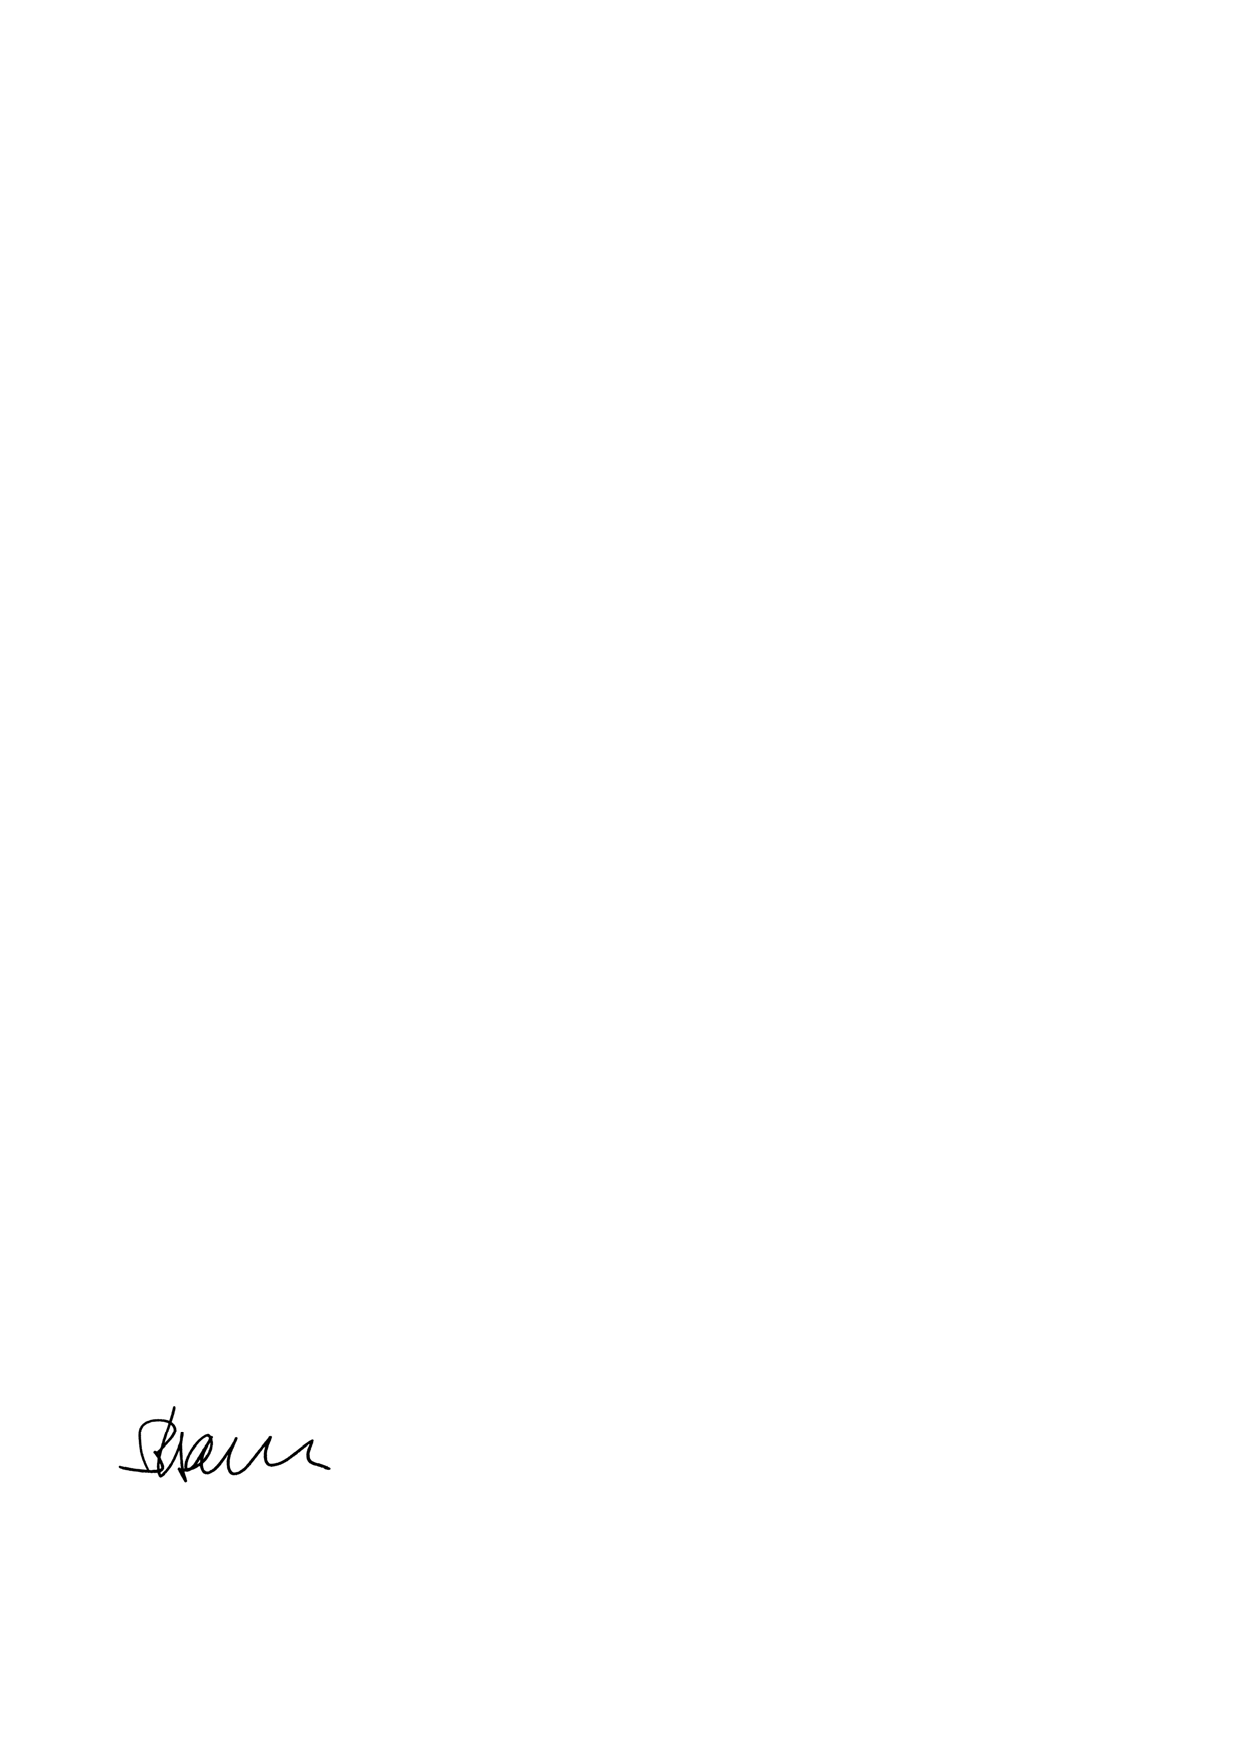
\includegraphics[width=4cm]{DeanSig}
 \end{figure}



Bernhard Kramer

\cleardoublepage
%\bibliographyunit[\subsection]
%\shorttitle{Information and Communication Technologies}
\section{Information and Communication Technologies}

The increasing impact of information and communication technology dominates our everyday
life, our society, and the environment.  Examples comprise the World-Wide-Web, the
ubiquitous use of computers, cellular multimedia and wireless communications, robots in
factories as well as in offices and homes, and sophisticated computer models used to
predict the evolution of complex systems such as the global climate.

The enormous level of integration in micro-electronics has enabled unprecedented progress
in many sectors -- and even more importantly, it has created many new profitable
technologies and services based on them. The 21st century will witness technologies that
enable machines to do things that have been so far restricted to humans: machines will be
able to sense, act, speak, listen, decide and sometimes understand. Our T-shirts may have
their own Internet addresses and wirelessly tell the laundry machine about proper
treatment. We will see cars that negotiate with each other in order to maximize traffic
flow while reducing pollution using sophisticated energy management systems. Manufacturing
technologies will improve using a combination of detectors and software to control
processes. Robots are also more and more used in domains where some autonomy and
intelligence is necessary. They work under conditions where it is unpleasant or even risky
for humans like in abandoned mines or at disaster sites and where they have to deal with
situations unforeseen by their designers and programmers. The hallmark of such smart
systems is their integration of technologies from analogue devices and sensors,
communication systems and networks, internet services, artificial intelligence, machine
learning, robotics, and many more.

The School of Engineering and Science actively contributes to this
rapidly growing, boldly interdisciplinary endeavor, focusing on the
areas described in the following.
%
%{\em{Mathematical and Symbolic Modeling}\\
%  \item Reasoning and Semantics
%  \item Simulation and Control of Complex Systems
%  \item Machine Learning
%  \end{itemize}
%\item {\em{Communication Networks and Systems}}, in particular:
%  \begin{itemize}
%  \item Wireless and Cellular Communications
%  \item Digital Transmission Methods and Coding
%  \item Networks and Protocols
%  \item Harmonic Analysis applied to communications engineering
%  \end{itemize}
%\item {\em{Robotics and Embedded Systems}}, in particular:
%  \begin{itemize}
%  \item Robotics
%  \item Applied Algorithms
%  \end{itemize}
%\item {\em{Knowledge and Information Management Systems}}, in
%  particular:
%  \begin{itemize}
%  \item Raster Data Services
%  \item Knowledge Management Systems
%  \item Distributed Systems
%  \item Hierarchical Data Representation
%  \end{itemize}
%\item {\em{Microelectronic Devices and Technologies}}, in particular:
%  \begin{itemize}
%  \item Electronic Devices and Nano Photonics
%  \item Microelectronics
%  \end{itemize}
%\item {\em{Digital Signal Processing}}, in particular:
%  \begin{itemize}
%  \item Signal Processing in Communications
%  \item Nonlinear Signal Processing and Control
%  \end{itemize}
%\end{enumerate}

%%% Local Variables:
%%% mode: latex
%%% TeX-master: "report"
%%% End:


%\input{./EECS/MathSymbol}
%\input{./EECS/Kohlhase_2005}
%\input{./EECS/Antoulas_2005}
%\input{./EECS/Jaeger_2005}

%\shorttitle{Communication Networks and Systems}
\subsection{Communication Networks and Systems}

The basic desire of modern society to be able to access and
distribute ``any'' information at ``anytime'' and ``anywhere'' is
the driving force for the rapid development of communication
networks and systems. The implications of these goals are manifold
and require truly interdisciplinary research efforts. A typical, but
clearly not complete, list of involved high level research fields
includes

\begin{myitemize}
\item Wireless Network Engineering and System Design
\item Network Interoperability
\item System capacity management and optimization
\item Information transmission
\item Network protocols 
\item Information security.
\end{myitemize}

All these research areas are strongly inter-related and the strength
of a research cluster in ``communication networks and systems''
resides in the close cooperation of the respected research groups
involved. The particular `flat hierarchy' at IUB (no departments and
chairs) fosters such cooperations.

%%% Local Variables:
%%% mode: stex
%%% TeX-master: "report"
%%% End:

%\input{./EECS/Haas_2005}
%\input{./EECS/Henkel_2005}
%\input{./EECS/Schoenwaelder_2005}
%\input{./EECS/Pfander_2005}

%\shorttitle{Robotics and Embedded Systems}%
\subsection{Robotics and Embedded Systems} %
Robotics is the driving force behind the increasing omnipresence
of automation, not only in industry but also in many areas of our
daily lives. In addition to their well-established role as
programmable machine-tools, robots are more and more used in
domains where some autonomy and intelligence is necessary, where
the system is not constantly supervised by a human operator and
where it has to be adaptive as the developer of the system can not
fully predict which situations the system will encounter in its
application environment. The related computer hardware and
software are the key ingredients of robots.

%%% Local Variables:
%%% mode: latex
%%% TeX-master: "report"
%%% End:

%\input{./EECS/Birk_2005}
%\input{./EECS/Carpin_2005}

%\shorttitle{Knowledge and Information Management Systems}
\subsection{Knowledge and Information Management Systems}


Today's information services are rapidly changing from statically served data to
information that is dynamically tailored to each individual user's current needs. This
information is fetched instantaneously from networked, distributed sources which
themselves change and evolve continually. At the same time, new representation formats
allow to discover and specify the internal and functional structure of information and
drive services that previously required (human) understanding. Technically, we observe the
convergence of databases, Internet, and distributed systems into semantically enriched
knowledge systems which allow the casual as well as the professional user to deal with the
ever-growing amount of information available.  Another issue is the presentation of
information to the user.  Data visualization is concerned with the management of large
data, the filtering and extraction of salient features, and their visual representation in
an expressive, intuitive, and interactive manner.

%%% Local Variables:
%%% mode: latex
%%% TeX-master: "report"
%%% End:

%\input{./EECS/Baumann_2005}
%\input{./EECS/Kohlhase2_2005}



%\shorttitle{Microelectronic Devices and Technologies}
\subsection{Microelectronic Devices and Technologies}

To continue the rate of progress in information and systems and
technologies into the next decade fundamental questions in material
science and manufacturing technology have to be answered to further
reduce the device dimension into the sub 100nm arena and increase
the complexity of integrated circuits. Novel Micro and Nano
Technologies are needed, either to overcome limitations to further
shrinking of devices and/or to implement novel electronic
hardware/services (such as large flexible displays). In parallel to
the development of novel devices, the integration into large volume
manufacturing processes and the specific problems associated to
manufacturing and quality/reliability engineering of these have to
be addressed, according to the principles of concurrent engineering.

%%% Local Variables:
%%% mode: latex
%%% TeX-master: "report"
%%% End:

%\input{./EECS/Knipp_2005}
%\input{./EECS/Bergholz_2005}
%\shorttitle{Digital Signal Processing}
%\subsection{Digital Signal Processing}
%\input{./EECS/Henkel2_2005}
%\input{./EECS/Haas2_2005}
%\input{./EECS/Jaeger2_2005}

%Life Sciences
%%%%%%%%%%%%%%%%%%%%%%%%%%%%%%%%%%%%%%%%%%%%%%%%%%%%%%%%%%%%%%%%%%%%%%
%\cleardoublepage
%\shorttitle{Life Sciences}
\section{Life Sciences}

\begin{figure*}[ht]
  \begin{center}
   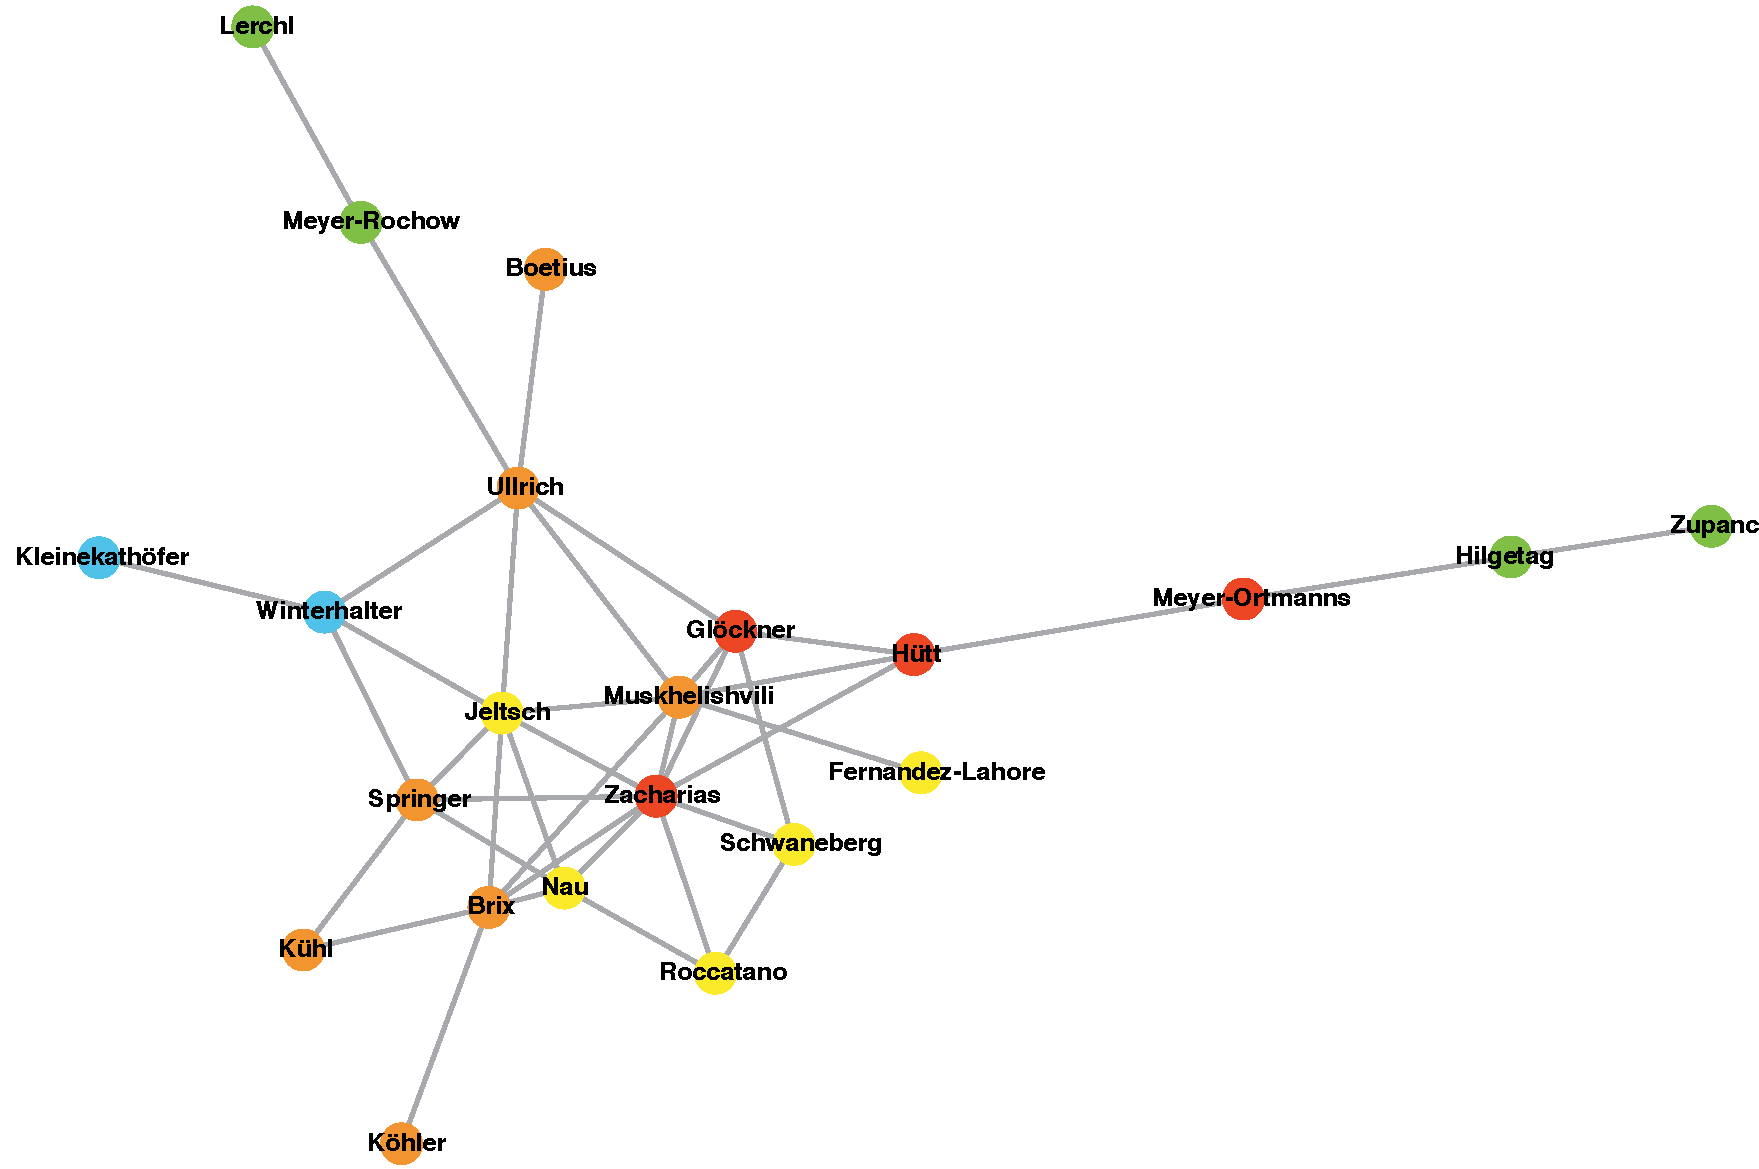
\includegraphics[width=\hsize]{network_LifeSci1_tmp03.pdf}
    \mycaption{Geometry and functionality of the complex biological network at Jacobs University Bremen that is formed by the interaction of Computational Biologists, Biophysicists, Biotechnologists, Neuroscientists, and Molecular Life Scientists.  }\label{fig:LifeSc}
   \end{center}
\end{figure*}


Life Scientists at IUB follow an integrated research approach that covers a variety of scientific fields and interests. The spectrum ranges from the analysis of molecules and their usage for biotechnological applications to the understanding of the mechanisms that explain the functions of complex systems like cells, organisms, and even entire habitat communities. Our research approaches combine experimental and theoretical work aiming towards future challenges in the target areas of the School of Engineering and Science. \\

The Life Scientists at IUB focus their research interests on
\begin{myitemize}
\item   the molecules and macromolecules which make up living matter,
\item the dynamical organization of genomes and cells,
\item   the biochemistry and physiology of life,
\item   the molecular mechanisms that maintain vital functions of cells, and
\item   the patho-physiological events which result in the onset of diseases.\\
\end{myitemize}


The research results provide us with insights into the molecular mechanisms that are found in microbes, plants and animals. Moreover, marine and terrestric habitats which are filled with life are analyzed in composition and interactivity. The perception of animals and human beings of their surrounding world is another important aspect of our research teams as is the modeling of complex systems like gene networks, metabolism, trafficking of molecules in cells, and interaction of living creatures in biological systems.\\

In 2006, a clear focus was on the spatial and temporal regulation of biological systems. Another important and recent advance is that the Molecular Life Scientists at IUB have filled their excellently designed and newly build research facilities and laboratories with life. Life Scientists at IUB have established numerous successful research collaborations within our research community. Above it, our research activities are embedded in the scientific communities of the Bremen-area and have attracted significant international attention. The nodes and edges that make up the units of the vital network of Life Scientists at IUB are illustrated in Figure \ref{fig:LifeSc}. \\




\textit{Perspectives}\\
The goal of the Life Scientists at IUB is to understand the function
of life, in its complexity and functional organization, on the
molecular and the systemic levels. We feel best prepared to further
evolve our research activities to face the major global challenges
of the future.


%\input{./LifeSciences/Biocomputing}
%\input{./LifeSciences/Gloeckner_2005}
%\input{./LifeSciences/Zacharias_2005}
%\input{./LifeSciences/Meyer-Ortmanns_2005}

%\shorttitle{Biotechnology}
\subsection{Biotechnology}

While within the Biophysics section, research attempts to understand the relation between protein structure and function and the Computational Biology studies place structural data into a systemic context, research in the Biotechnology section is about the \textit{design} of function.\\

Here the research activities range from enzyme design and directed protein evolution to large-scale screening for functional properties and molecular modeling as a route towards bioengineering.\\

In this form Biotechnology research at International University Bremen successfully addresses target areas ranging from energy and materials to water and food, as well as health. The wide variety of 2006 highlights demonstrate impressively the impact Biotechnology research at Jacobs already has on these target areas. These highlights include intense and successful joint projects with industry, several patents, substantial progress in carrying gene silencing technology to human cell lines and proofs of principle to several biotechnological and bioengineering concepts.\\

%\input{./LifeSciences/Jeltsch_2005}
%\input{./LifeSciences/Fernandez-Lahore_2005}
%\input{./LifeSciences/Schwaneberg_2005}
%\input{./LifeSciences/Winterhalter_2005}
%\input{./LifeSciences/Zakhartsev_2005}

%\shorttitle{Molecular Life Sciences}
\subsection{Molecular Life Sciences}
\label{MolLifeSc}

The Molecular Life Scientists at International University Bremen devote their research activities to the understanding of macromolecules and of the biochemical pathways which build up the units of life - our cells. The integration of cellular functions in the broader context of natural biological systems is an important aim of the research groups involved. A strong focus is set out to uncover the molecular mechanisms which maintain vital functions of healthy life. Hence, main expertise and research activities of Molecular Life Scientists are in the field of Molecular Medicine. The aim is to identify targets for drug design for the development of better treatments and therapies of diseases which challenge the modern world.\\

Our motivation is to combine basic sciences, modeling and simulation approaches, biochemical, cell and molecular biological approaches, assays employing organismic model systems as well as analyses of environmental habitats in order to answer key questions concerning the organisms of all divisions of life. \\

Key-questions of the research groups of the Molecular Life Sciences
at IUB comprise the understanding of
\begin{myitemize}
\item   DNA methylation as an important regulator for gene expression in bacteria and mammals,
\item   the concerted rearrangements of gene expression during growth and development,
\item   the significance of protein degradation for proper function of epithelial organs in adult mammalian organisms,
\item   the importance of brain glial cells for development of neurodegenerative diseases,
\item   the molecular mechanisms of the anti-viral immune response,
\item   the importance of virulence factors of plants during their response against  phytopathogens,
\item   molecular interactions of marine bacteria with each other and with phytoplankton cells,
\item   characteristics of diverse microbial habitats in the ocean, and
\item   the interaction of chemicals with marine life for the identification of biomarkers to predict toxic effects.\\
\end{myitemize}


Centrally important are the interactions between the groups that allow us to study molecular mechanisms and to deduce principles which are of significance for the complexity of all biological systems. Underlying principles governing gene expression and hence, proliferation and differentiation of cells are covered to a comparable extent as principles regulating the interaction of microbes, plants, and animals that live in terrestric and marine habitats.\\

%\input{./LifeSciences/Brix_2005}
%\input{./LifeSciences/Jeltsch_2_2005}
%\input{./LifeSciences/Springer_2005}
%\input{./LifeSciences/Kuehl_2005}
%\input{./LifeSciences/Muskhelishvili_2005}
%\input{./LifeSciences/Nau_2005}
%\input{./LifeSciences/Ullrich_2005}

%\input{./LifeSciences/NeuroPhysio}
%\input{./LifeSciences/Boetius_2005}
%\input{./LifeSciences/Hilgetag_2005}
%\input{./LifeSciences/Meyer-Rochow_2005}
%\input{./LifeSciences/Zupanc_2005}
%\input{./LifeSciences/Facilities}

%\cleardoublepage \shorttitle{Geosciences and Astrophysics}
%\input{./GeoAstro/Intro_GeoAstro}
\shorttitle{Geochemistry}
\subsection{Geochemistry}
%\input{./GeoAstro/Bau_2005}
\begin{bibunit}[plain]
\subsubsection{Marine Geochemistry}
\index{Koschinsky, Andrea}

\paragraph{Research Team}
Andrea Koschinsky (Professor), Herwig Marbler (Post-doc),
Thomas Schirmer (Post-doc), Jule Mawick (lab technician), Daniela
Mei\ss ner (lab technician), Katja Schmidt (PhD Student), Cristiane Jost
(DAAD exchange PhD student), Aryani Sumoondur (MSc student), Prasesh
Sharma (MSc student) \\

The research activity in the field of marine geochemistry continued in
2006 with its focus on marine hydrothermal systems as part of the DFG
Special Priority program SPP 1144: \quotedblbase{}From Mantle to
Ocean: Energy-, Material- and Life Cycles at Spreading Axes``. The
objective of the priority program is to quantify the processes at the
mid-ocean ridges from geological and biological investigations. The
target areas of this program are the Mid-Atlantic Ridge (MAR) at 15$^\circ$N
and 4$^\circ$-11$^\circ$S. The project of the IUB geochemistry group is entitled
\quotedblbase{}Hydrothermal Fluids at the Mid-Atlantic Ridge as Media
for the Transport of Energy and Mass from the Crust into the Hydro-
and Biosphere``. The second 2-years term of this project has started
in October 2005.

Apart from the hydrothermal research, our activities on experimental
and theoretical investigations of interactions between dissolved
metals, mineral phases and biota in the marine systems were
continued. New activities in the field of marine mineral resources
have been started.

\paragraph{Highlights}
The highlight of the hydrothermal research was cruise M68/1 with R/V
Meteor, where A. Koschinsky was chief scientist. This cruise continued
exploration for hydrothermal fields on the southern Mid-Atlantic
Ridge, which had been started as part of the SPP 1144 in 2005. Besides
the revisit of hydrothermal fields discovered the year before, the
combined use of an autonomous underwater vehicle AUV ABE from the
Woods Hole Oceanographic Institution and the remotely operated vehicle
ROV Quest from Marum, Univ. Bremen enabled the discovery of another 8
hydrothermally active sites in the area between 4 and
10$^\circ$S. Temperature measurements of fluids in the young volcanic
system at 5$^\circ$S revealed the highest temperature ever measured so
far in a hydrothermal fluid: 407$^\circ$C. At 3000 m, the water depth
of the vent site, this point represents the so-called critical point
of seawater, which separates the subcritical from the supercritical
fluid range. Gas bubbles and depleted salinity indicate ``boiling''
and phase separation. While this system is clearly characterized by
subsurface leaching of basaltic rock, the newly discovered site at
8$^\circ$S shows clear signatures of mantle rocks, underlining the
importance of ultramafic-hosted (mantle-rock hosted) hydrothermal
systems on slow spreading ridges such as the Mid-Atlantic Ridge.

Further investigation of organic metal complexation in hydrothermal
fluids confirmed our preliminary data, that toxic metals such as
copper are largely controlled by binding to organic ligands. This
probably makes them less bioavailable. Metal analyses of organic
tissue of hydrothermal mussels are carried out to compare how fluid
chemistry is reflected in the uptake of heavy metals by the organisms.

Laboratory experiments with trace metals and mineral particles in
seawater enhance our understanding in how the reactivity,
bioavailability and enrichment of rare metals in marine mineral deposits
are controlled. Sorption experiments with germanium, an element of
interest for semiconductor technologies, has shown a preferential
uptake on Fe-oxide containing precipitates. Similar results were
obtained for tellurium.  A newly started DFG project on tellurium and
selenium in geochemical systems in its first phase focuses on the
development of sensitive analytical techniques for these trace
elements in natural water and rock samples.

The increasing global demand for mineral resources has revived
interest in marine minerals, such as manganese nodules. In a project
funded by the BGR Hannover (German Geological Survey), the abundances
of rare valuable metals in marine manganese nodules are investigated
by literature search and chemical analyses in our geochemistry lab. As
in the past the economic interest was mostly based on metals such as
copper, nickel, zinc, and cobalt, there is a lack of reliable data for
valuable trace elements, including platinum group elements, rare earth
elements, and others.
%\nocite{koschinsky1}

\nocite{koschinsky1}\nocite{koschinsky2}\nocite{koschinsky3}


\begin{figure}[ht]
  \begin{center}
    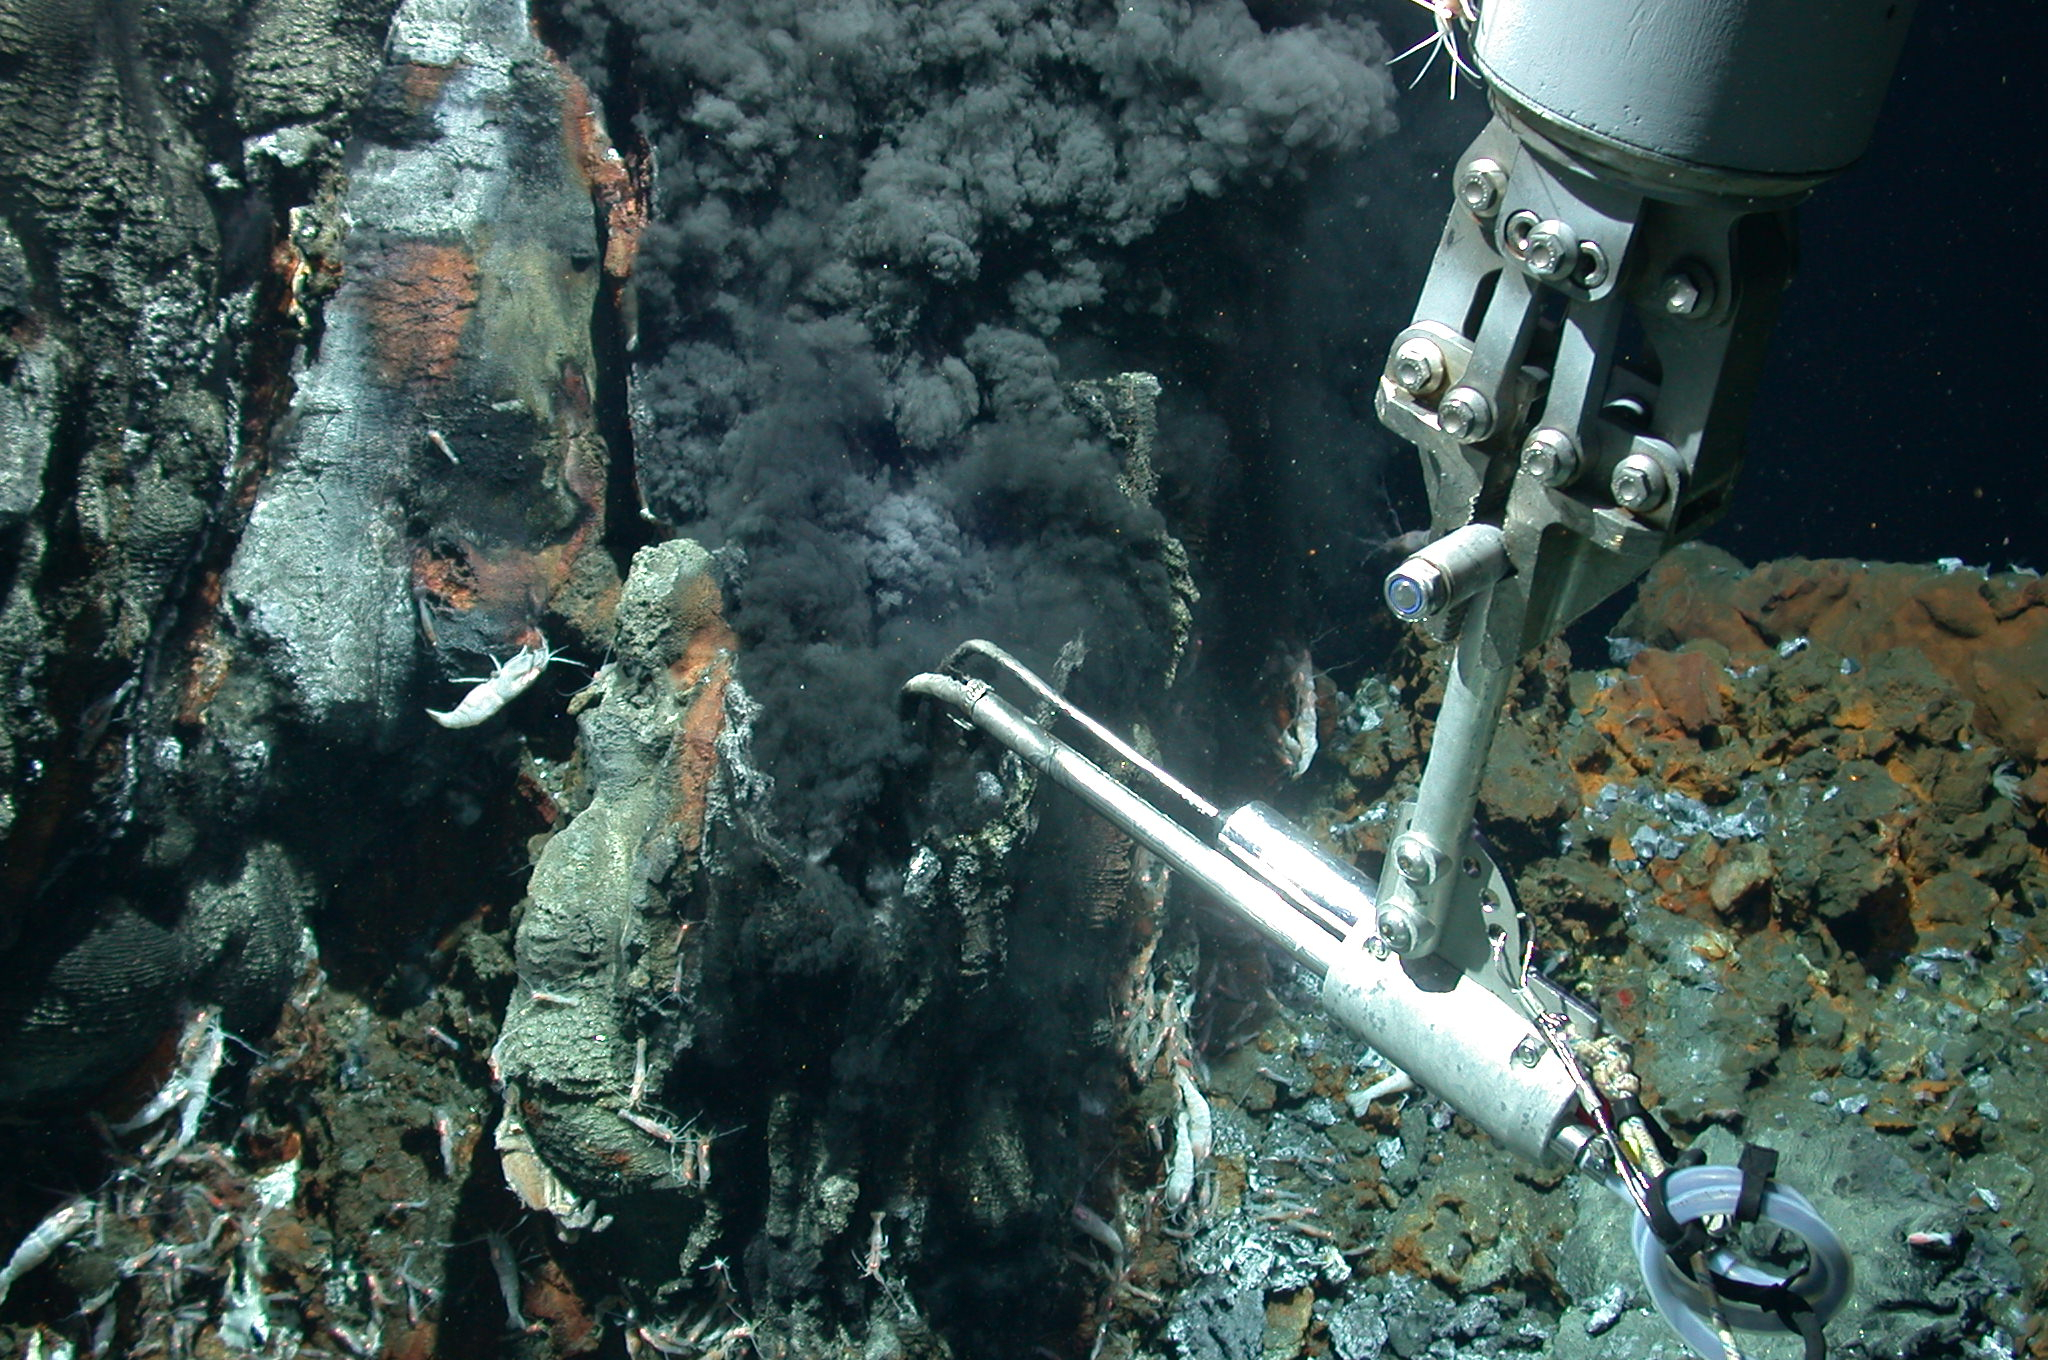
\includegraphics[width=\hsize]{GeoAstro/Koschinsky/Koschinsky_2006_Fig.png}
    \mycaption{Sampling of the hottest hydrothermal vent fluid found so far (407$^\circ$C) at 5$^\circ$S on the Mid-Atlantic Ridge during cruise M68/1. The fluid is taken with the KIPS fluid sampling system equipped with a temperature sensor. (Picture copyright: MARUM, Univ. Bremen)  )}\label{fig:profxxx}
   \end{center}
\end{figure}

\newpage
\paragraph{Collaborations}
\noindent

Regional:
\begin{enumerate}
\item {\sl International University Bremen}\\ Prof. Dr. M. Bau
\item {\sl Universit\"at Kiel}\\Dr. Dieter Garbe-Sch\"onberg
\item {\sl Univ. Hamburg}\\Dr. Richard Seifert
\item {\sl MPI Bremen} \\ Dr. Christian Borowski, Dr. Nicole
Dubilier
\item {\sl BGR Hannover} \\ Dr. Christian Ostertag-Henning, Dr. Thomas
Pletsch, Dr. Thomas Oberth\"ur, BGR
Hannover
\item {\sl Universit\"at Bremen, MARUM}\\ Dr. Volker Ratmeyer, Christian
Seiter
\end{enumerate}

National:
\begin{enumerate}
\item {\sl Univ. M\"unster} \\ Prof. Dr. Harald Strau\ss
\end{enumerate}

International:
\begin{enumerate}
\item {\sl US Geological Survey, Menlo Park, CA}\\ Dr. James Hein
\item {\sl University of Otago, New Zealand}\\ Dr. Sylvia Sander
\item {\sl Universidade de Santa Maria, Brazil} \\ Prof. Dr. Leandro
de Carvalho
\item {\sl Woods Hole Oceanographic Institution, MA}\\ Dr. Chris
German
\end{enumerate}


\paragraph{Grants}
% list the running grants in 2005, if none have been received, please delete this
% subsection.
\begin{enumerate}
\item
Funded by DFG, \emph{Vom Mantel zum Ozean: Stoff-, Engergie- und Lebenszyklen an
  Spreizungsachsen},  KO 2310/2-3,  P.I.: {A.Koschinsky} (November 2005 - July 2008)

\item
Funded by DFG, \emph{Die redoxabh\"angige Fraktionierung von Selen und Tellur in
  geochemischen Systemen\dots}, KO 2906/4-1, P.I.: {A. Koschinsky, } M. Bau, (September
2006 - September 2008)
 
\item
Funded by BGR (Bundesanstalt f\"ur Geowissenschaften und Rohstoffe) Hannover,
\emph{Literaturstudie Manganknollen}, (September 2006 - April 2007)

\item
Funded by DAAD, \emph{PROBRAL exchange program with Brazil. Speciation of
elements of clinical and environmental relevance in saline fluids}, DAAD Project
no. 415-br-PROBRAL/po-D/05/30366, (January 2006 - December 2007)

%\paragraph{References}
%\bibliography{combined}
\end{enumerate}

\putbib[combined]
\end{bibunit}
%\shorttitle{Marine Geology and Geophysics}
%\subsection{Marine Geology and Geophysics}
%\input{./GeoAstro/Thomsen_2005}
%\input{./GeoAstro/Unnithan_2005}
\shorttitle{Computational Space and Astrophysics}
\subsection{Computational Space and Astrophysics}
\begin{bibunit}[plain]
%\documentclass[twocolumn]{article}
%\usepackage{graphicx}
%\begin{document}
%%% comments begin with a % sign.

\subsubsection{High-energy astrophysics, computational fluid mechanics}
\label{GeoAstro:Bruggen}
\paragraph{Research Team:}
Marcus Br\"uggen (Professor), Elke R\"odiger (Postdoc), Matthias Hoeft
(Postdoc), Thomas  Guimbretiere (PhD student)

%%% give a very short (150 words description of your research area)

My research is concerned with issues in the areas of astrophysical and
computational fluid mechanics, high-energy astrophysics and solar
physics.  Many topics of my research cover a wide range of scales -
from the propagation of waves in the Sun to the dynamics of flows in
galaxies and clusters of galaxies. The macroscopic flows have typical
scales of thousands of kilometers, for instance in stars, to many
thousands of light years in galaxies and clusters of galaxies. These
macroscopic flows are coupled to microscopic processes, such as
viscosity, nuclear flame fronts or radiative processes that take place
on scales of centimetres or lower. It is the major challenge of the
coming years to bridge this huge span in scales which cannot be
resolved by greater computer power alone. Novel algorithms and
numerical techniques have to be invented to model the interactions
between processes on such different scales.


\paragraph{Highlights}

%%% give a short (500 words)description of the research highlights. 1 figure costs 100 words


\noindent Recent observations show a multitude of physical effects
that occur when powerful jets launched by supermassive black holes
interact with the surrounding medium. While these effects are widely
believed to be crucial for the formation of structure in the universe,
they are still poorly understood. Clusters of galaxies are excellent laboratories for studying the
  interaction between active galactic nuclei (AGN) and
  diffuse gas.  Recent observational evidence demonstrates that
  the lives of AGN and their environment are
  closely intertwined. This complex pattern of processes calls for a combined approach of simulations and detailed diagnostics of observations.\\

\noindent Here the main questions are: How is the energy of the jet
dissipated in the intracluster medium (ICM)? How are bubbles, ripples
and waves produced?  What determines the variability of the jet? Is
heating by jets in active galactic nuclei (AGN) universal? How does
feedback operate? What is the kinetic energy output of the AGN? What
is the fate of the ghost bubbles?\\

\noindent Using sophisticated simulations on massively parallel
computers at the National Center for Supercomputing Applications (USA)
and at the Forschungszentrum J\"ulich, we have shown that jets
launched by black holes can prevent the catastrophic cooling in the
centres of galaxies. This project is supported by a recently awarded DFG grant within the
Schwerpunkt 'Witnesses of Cosmic History' supporting a postdoc and a
PhD student.\\

\noindent Moreover, in the past year, we have achieved the following:

\begin{itemize}

\item We have studied the interaction of the jet with its environment, for the first time taking into account the dynamic nature of the cluster gas.  The simulations successfully reproduce the observed morphologies of radio sources in clusters.  We find that cluster inhomogeneities and large-scale flows have significant impact on the morphology of the radio source.

\item With the X-ray telescope XMM-Newton, we have made the deepest observations of the nearest jet from a supermassive black hole and its surroundings. We have identified shock waves and other physical processes in the vicinity of the black hole. We found several new features in M87 related to heating mechanisms of the ICM.

\item When galaxies move through the universe, they experience a head wind. This head wind  can remove the chemical elements that are synthesized in the stars from the gravitational well of the galaxy and disperse it through the universe. The efficiency of this process is unknown, but very important as it influences subsequent structure formation. We produced sophisticated computer models in 3D to determine this efficiency.

\item We have investigated the role of AGN in forming the broad metal abundance peaks observed in cool core clusters. To this end, we carried out numerical simulations that modelled the interplay between metal injection from the central galaxy and the AGN-blown cavities. The resulting distribution patterns were compared to observations.

\item The ICM has a metallicity of about 1/3 solar. However, cooling core clusters,
i.e. clusters with a centrally peaked X-ray brightness, show peaked abundance
profiles. A number of observations indicates that supernovae in the central galaxy
are mainly responsible for the metal enrichment in the central part of
clusters. However, the observed metallicity profiles are much broader than the
light profiles of the central cluster galaxy. Hence, the difference in the
light and the metal distributions are interpreted as the result of transport
processes that have mixed metals into the ICM. We have characterised the AGN-ICM interaction effects by means of deep X-ray observations of nearby clusters, in particular with M87. While it appears to be established that the metals produced by the central galaxy are dispersed into the ICM to form the
broad abundance peaks, it remains unclear what the mechanism is via which the
metals are transported. As one likely mechanism, we studied the effect of AGN-inflated bubbles that rise buoyantly and lift metal-rich gas upwards. We demonstrated that AGN can account for the distribution of metals in clusters of galaxies.

\end{itemize}

% to include a figure, generate a file xxx.pdf and integrate the following lines
\begin{figure}[ht]
  \begin{center}
    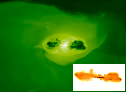
\includegraphics[width=\hsize]{/Bruggen/Brueggen_2006_Fig.png}
    \caption{Snapshots of the gas density in a simulation of a jet in a cluster of
galaxies. One can see how the jet drives shocks into the intracluster
medium. The inset shows the simulated radio emission from this jet.}
    \label{fig:xxx}
  \end{center}
\end{figure}
% to reference it use ``Figure.~\ref{fig:xxx}''; the numbers will be computed automatically.


\paragraph{Organization}
% list the (research) events you have organized, if any,

\begin{enumerate}
\item Tagung des "Rat deutscher Sternwarten", 18. Sep. 2006, IUB
\item Organisation eines DFG Rundgespr\"achs "Astrophysik-Schwerpunkte", 21.-22. Sep. 2006 in Garching
\end{enumerate}

\paragraph{Collaborations}
\begin{enumerate}
\item {\sl University of Colorado}\\ Prof. Markusz Ruszkowski,
  Dr. Eric Hallman,  Prof. Jack Burns
\item {\sl University of Wisconsin}\\ Prof. Sebastian Heinz 
\item {\sl Sterrewacht Leiden}\\ Prof. Joop Schaye and Dr. Claudio
  Dalla Vecchia 
\item {\sl MPI f\"ur Extraterrestrische Physik}\\ Prof. Hans
  B\"ohringer and Dr. Eugene Churazov
\item {\sl Stanford University}\\ Prof. Tom Abel (Stanford)
\item {\sl Los Alamos National Laboratory}\\ Dr. Brian O'Shea (LANL)
\end{enumerate}

\paragraph{Grants}
% list the running grants in 2005, if none have been received, please delete this
% subsection.
\begin{enumerate}

\item Interactions between Active Galactic Nuclei and the Intracluster Medium
(BR 2026/3-1)

\item The CME source region in LOFAR-related simulations (VO 855/2)

\end{enumerate}
\nocite{2006astro.ph.10874S}
\nocite{2006MNRAS.371..609R}
\nocite{2006astro.ph..9831H}
\nocite{2006MNRAS.369..567R}
\nocite{2006astro.ph..6664H}
\nocite{2006AN....327..587B}

% list the publications of 2005 (also accepted and in press), if none have been received, plese delete this
% subsection. Enter the publications into the SES publications database at
% http://kwarc.eecs.iu-bremen.de/ses-pubs/index.php and only reference them here.

%\begin{description}
%  \item[Journals] Nature~\cite{Kohlhase:Nature}, Science~\cite{Kohlhase:Science}
%  \item[Conference Proceedings] CADE~\cite{Kohlhase:CADE1}, ...
%  \item[Books/Collections] \ldots
%\end{description}
%\end{document}

%%% Local Variables:
%%% mode: latex
%%% TeX-master: "RP-EECS"
%%% End:

\putbib[combined]
\end{bibunit}
%\input{./GeoAstro/Rosswog_2005}
\begin{bibunit}[plain]

\subsubsection{Space plasma physics}
\index{Vogt, Joachim}
\label{GeoAstro:Vogt}

\paragraph{Research Team}
Dr. Joachim Vogt (Professor), Dr. Bertalan Zieger,
Dr. Matthias Hoeft (since August 2006)\\

The structure and dynamics of near-Earth space are controlled
by the interaction of the geomagnetic field with the stream
of solar particles called the solar wind.  This interaction
leads to the formation of a magnetic cavity in space that is
commonly referred to as the Earth's magnetosphere.  The highly variable
solar wind causes magnetospheric dynamics on short timescales of hours
to days which leads to space weather phenomena like geomagnetic
storms, auroral emissions, failures of communication satellites, and
electrical power disruptions on the ground.  On geological timescales,
variations of the geomagnetic core field are expected to have
a strong effect on the magnetospheric structure and on the behaviour of
energetic particles in near-Earth space.  At IUB, magnetosphere formation
and other space plasma processes are studied using large-scale
magnetohydrodynamic (MHD) simulations, plasma theory, and data
from spacecraft.


\paragraph{Highlights}

The DFG funded project \emph{Studies of paleomagnetospheric processes\/}
dealt with the magnetosphere during geomagnetic polarity transition periods.
In a paper published in the Journal of Geophysical Research, MHD simulation
results were compared with an empirical model for the size and the shape
of the magnetospheric boundary layer (magnetopause).  Very good agreement
was found within the validity range of the empirical model.  Outside this
range our MHD simulations offer a more complete description of the
magnetopause shape and size in terms of solar wind parameters and the
geomagnetic dipole moment.  The empirical model could be generalized
beyond the former validity range.
In a second study, the distribution of energetic particles in the
paleomagnetosphere was investigated by analytical means.  Since our
collaborators at the universities in Bremen and Osnabr{\"u}ck use our
results as input to model the chemistry of the middle atmosphere in
response to solar energetic particle events, we were particularly
interested in the polar cap region that is most affected by such
particle events.  Our results indicate that with decreasing dipole
moment and increasing quadrupole contribution, this region can extend
down to latitudes as low as 40 degrees.
More complex magnetic field configurations are modelled using
MHD simulation results and field line tracing schemes.
Figure~\ref{fig:Vogt_2006_Fig} illustrates how the open field line
region may look like during a geomagnetic polarity transition with a
highly non-axisymmetric core field.  An invited paper on the results
of this project and on the work of our collaborators within the
DFG Priority Programme SPP 1097 was presented at a DFG Colloquium.

\begin{figure}[ht]
  \begin{center}
    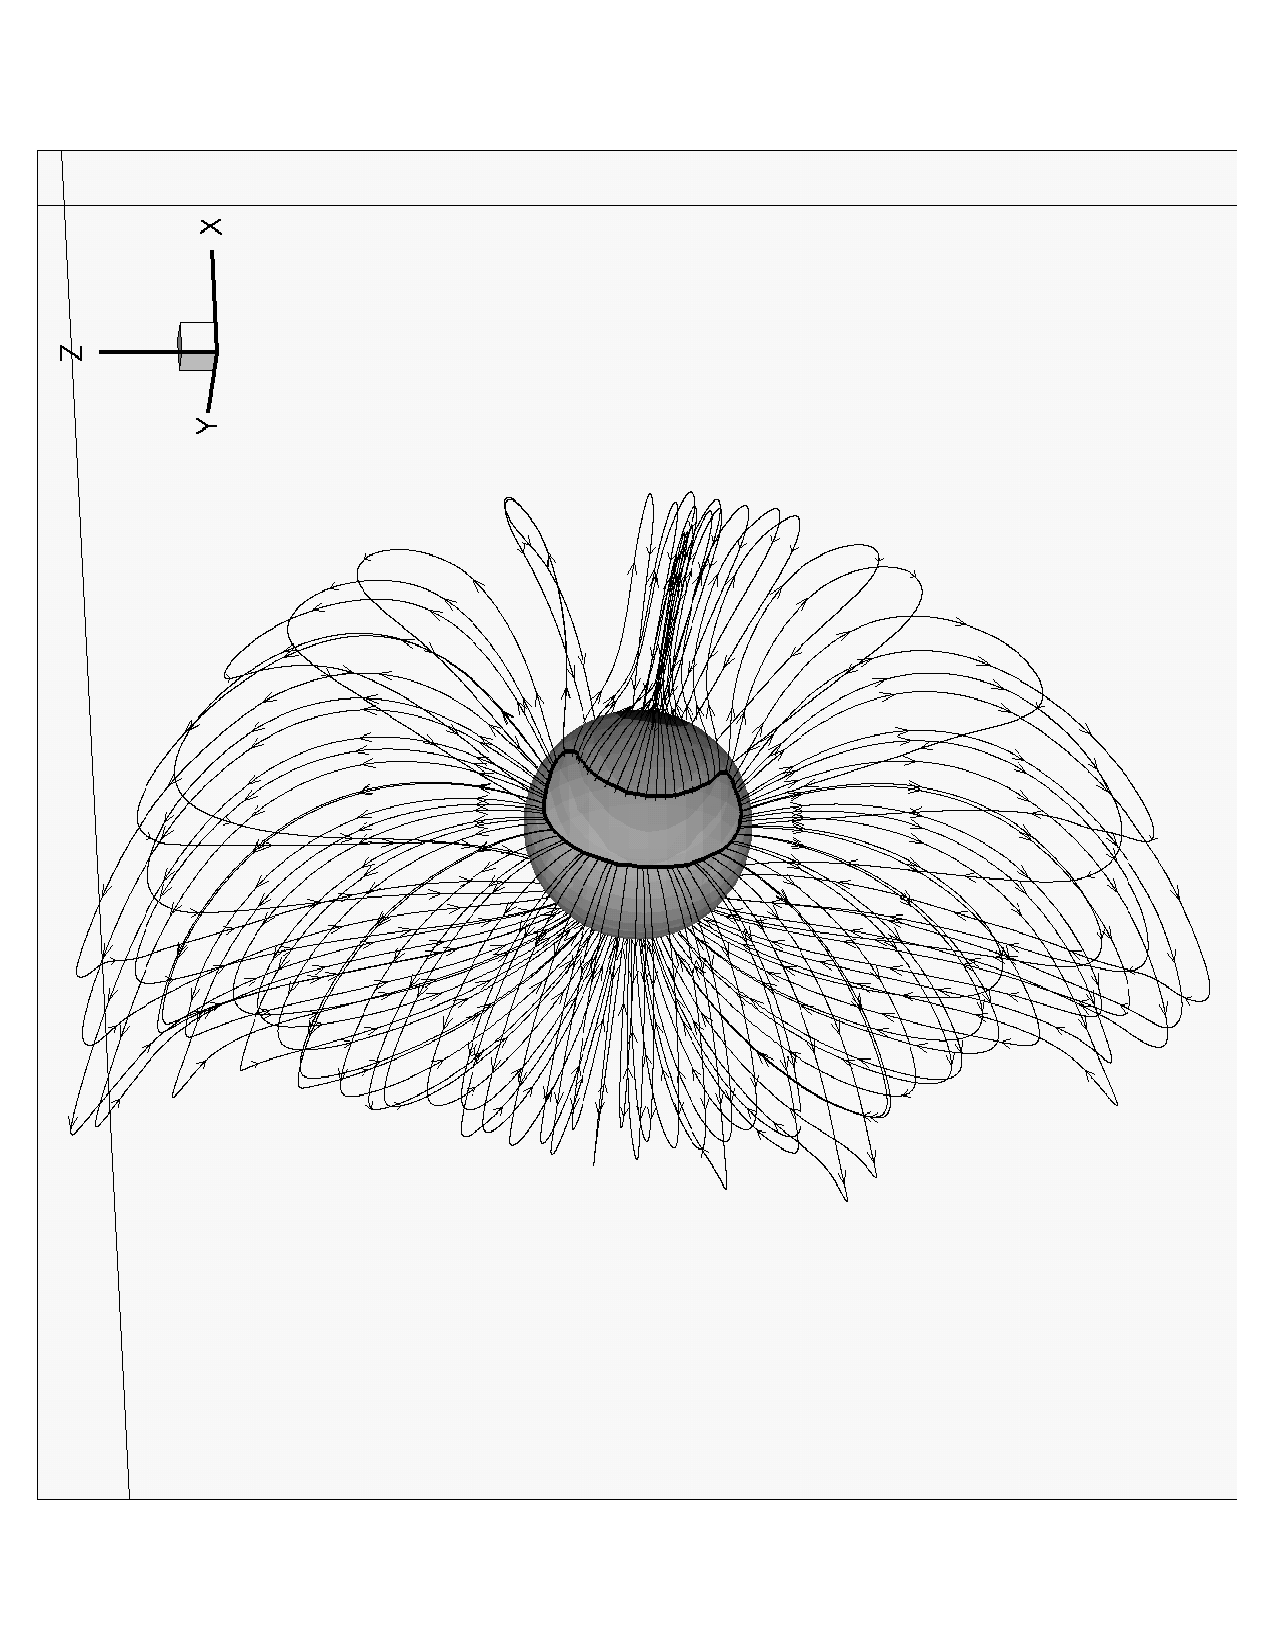
\includegraphics[height=\hsize, angle=270]{Vogt/Vogt_2006_Fig}
    \mycaption{Closed magnetic field lines in a simulated paleomagnetosphere.
               The region in the center is penetrated by open field lines
               (not shown) and thus accessible by low-rigidity particles
               from solar energetic particle events.  Figure produced
               by Bertalan Zieger.}
    \label{fig:Vogt_2006_Fig}
  \end{center}
\end{figure}

In a second DFG funded space plasma project (jointly with Prof. Marcus
Br{\"u}ggen and Dr. Matthias Hoeft), we are planning to model radio emissions
of coronal mass ejections which happen on time scales like hours or days,
and lead to space weather phenomena like geomagnetic storms and substorms.
The project started in August 2006.

Supervised jointly by faculty from marine geosciences (Prof. Laurenz
Thomsen) and space physics (Prof. Joachim Vogt), the GeoAstro student team
\emph{Neptunas\/} participated in ESA's Student Parabolic Flight Campaign
2006.  During two parabolic flights on the Zero-G Airbus A-300,
four 3rd-year students Simona Balan, Matteo Kausch, Eva St\"ueken, and
Wilken-Jon von Appen studied the influence of microcravity on the
photosynthetic yield of microalgae.  The students received support also
from industry (OHB System, Bluebiotech, Heinz Walz GmbH).



\paragraph{Organization}

\begin{enumerate}
\item
COSPAR Capacity Building Workshop to be held in June 2007, Sinaia, Romania
(jointly organized with Prof. Peter Willmore, University of Birmingham,
Prof. Thierry Dudok de Wit, CNRS Orleans, Dr. Octav Marghitu, MPE Garching
and ISS Magurele, Dr. Marius Echim, BIRA Bruxelles and ISS Magurele).
Sponsored by COSPAR, ROSA, and other space organisations.
\item
Successful WAP proposal to renew the computational infrastructure of the
CLAMV Teaching Lab (jointly with Prof. Martin Zacharias, Dr. Achim Gelessus,
and Dr. Heinrich Stamerjohanns).
\end{enumerate}


\paragraph{Collaborations}\noindent

Regional:
\begin{enumerate}
\item
{\sl Technische Universit{\"a}t Braunschweig}\\
Prof. Karl-Heinz Glassmeier
\item
{\sl International University Bremen}\\ Prof. Marcus Br{\"u}ggen,
Prof. Laurenz Thomsen, Prof. Vikram Unnithan
\item
{\sl Universit{\"a}t Osnabr{\"u}ck}\\
Prof. May-Britt Kallenrode
\item
{\sl Universit{\"a}t Bremen}\\
Dr. Miriam Sinnhuber
\item
{\sl OHB-System, Bremen}\\ Dr. Klaus Slenzka
\end{enumerate}

National:
\begin{enumerate}
\item
{\sl Ruhr-Universit{\"a}t Bochum}\\
Prof. Reinhard Schlickeiser, Priv.-Doz. Dr. Horst Fichtner
\end{enumerate}

International:
\begin{enumerate}
\item
{\sl University of Michigan, Ann Arbor, USA}\\
Prof. Tamas Gombosi, Dr. Ward Manchester
\item
{\sl ASTRON, The Netherlands}\\ Dr. Michiel van Haarlem
\end{enumerate}


\paragraph{Grants}

\begin{enumerate}
\item
Funded by DFG, \emph{Studies of paleomagnetospheric processes}
(October 2004 - December 2006)
\item
Funded by DFG, \emph{The CME source region in LOFAR related
simulations} (January 2006 - March 2008)
\end{enumerate}

\paragraph{Other Support Grants}
\begin{enumerate}
\item Support from the European Space Agency (ESA) and from
industry (OHB System, Bluebiotech, Heinz Walz GmbH) for the GeoAstro
student team \emph{Neptunas\/} to participate in the \emph{ESA
Student Parabolic Flight Campaign 2006\/}.
\end{enumerate}
\nocite{vogt:terra-nostra-vogt-etal-2006}
\nocite{vogt:asr-zieger-etal-2006}
\nocite{vogt:jgr-zieger-etal-2006}

\putbib[combined]
\end{bibunit}
%\cleardoublepage
% \shorttitle{Molecular Electronics and Dynamics}
%\input{./Nano/Introduction_Nanoscience}
%\input{./Nano/Knipp_2005}
%\input{./Nano/Rohlfing_2005}
%\input{./Nano/Tautz_2005}
%\input{./Nano/Wagner_2005}

%\cleardoublepage
% \shorttitle{Novel Materials}
%\input{./Nano/Kortz_2005}
%\input{./Nano/Nugent_2005}
%\input{./Nano/Materny_2005}
%\input{./Nano/Richards_2005}

\cleardoublepage
% \shorttitle{Bionanotechnology}
%\input{./Nano/Nau_2005}
%\input{./Nano/Fritz_2005}
%\input{./Nano/Winterhalter_2005}

\cleardoublepage
%\section{An Introduction from the Dean} \shorttitle{The Jacobs Center for Lifelong Learning and Institutional Development}

Western industrialized nations have been undergoing fundamental changes in economic, cultural and social life. These changes are precipitated by more and more people reaching old and very old age, by markedly reduced birth rates, by living in an era of rapid knowledge turnover and by ever increasing globalization. Consequently, patterns of working, learning, and living need to change apace. This implies challenges for social institutions, including institutions of higher education, for corporations as well as for the individual. It is the goal of the Jacobs Center of Lifelong Learning and Institutional Development (JCLL) to do \textit{research} that contributes to the knowledge necessary to optimize the current transformations, and to provide \textit{education} and \textit{consulting} that support these transformations. Against the background of this historic constellation, the JCLL pursues the general aim to better understand individual and institutional conditions of \textit{productive adult development} and it does so from a systemic perspective (see below). Productive is defined in a broad sense that goes beyond the narrow economic understanding of productivity as exclusively linked to the contribution to the gross national product (cf. Staudinger, 1996).

%Over the past years, ``lifelong learning'' has become a rather overworked catchphrase, and sometimes even an empty shell. However, with regard to the current changes in Western industrialized societies, it has become more and more important for the individual and corporations alike to be able to continuously adapt to changing circumstances and environments. At the JCLL we have therefore opted for a definition of lifelong learning as one of three central developmental mechanisms, the other two being maturation/senescence and action. Learning in this sense encompasses formal as well as informal and incidental learning episodes. It addresses the knowledge and skills that are needed in personal, civic, social and professional life. Investigating lifelong learning at the JCLL is therefore part and parcel of the study of lifespan development. 


%The notion of lifelong learning within JCLL thus rests on Wilhelm von Humboldt's idea of education that is neither restricted to the learning of facts nor to learning in school. Humboldt proposed a notion of education that concerns the whole life course and all spheres of life. His notion of education also includes education in the sense of working on personality growth and maturation as well as the establishment of a value system that aims to not only further one's own good but also the common goal. This notion of ``Bildung'' (which is not properly captured by the English term education) and lifelong learning is very closely linked to the idea of optimizing human development in the sense of positive lives.
%\enlargethispage*{0.2cm}

%The JCLL \looseness=-1 focuses in its research on the analysis of \textit{development in context} and more specifically in the work context. By investigating human and organizational development in the work context, we aim to understand how individual (body and mind) and institutional conditions interact to produce outcomes on the individual as well as the organizational level. Interactionism forms the basis of our systemic model of adult development in the work context (see Figure \ref{fig:deanIntro}). Located in its center is the developing (aging) individual. In our model, we acknowledge that the individual as smallest system unit already comprises two dimensions: a mechanic and a pragmatic dimension (cf. Staudinger \& Pasupathi, 2000). 


%\begin{figure}[h]
 % \begin{center}
  %  \resizebox{0.5\textwidth}{!}{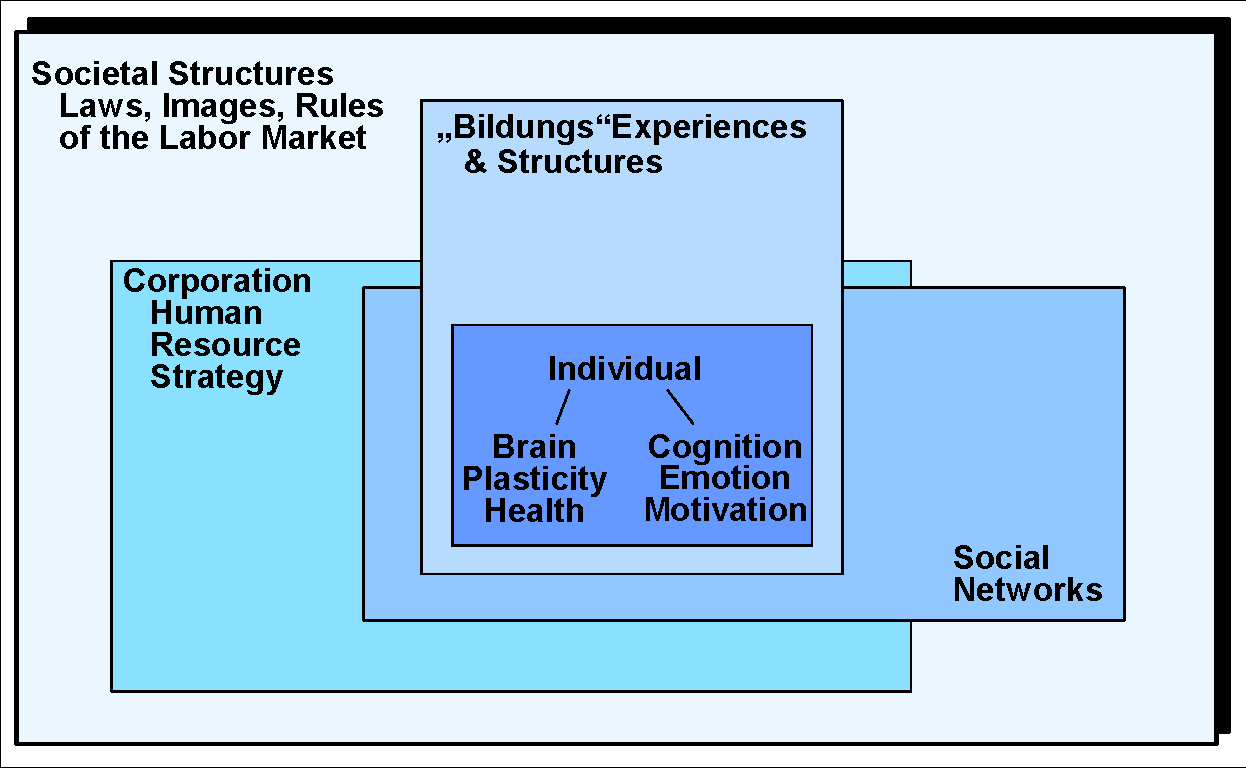
\includegraphics{deanUrsulaStaudingerIntro}}
   % \caption{Productive adult development at the Jacobs Center: A systemic approach (based on Staudinger, 2006).}
   % \label{fig:deanIntro}
  %\end{center}
%\end{figure}


\newpage
%The mechanic dimension refers to the fact that we all are biological beings with regard to our intelligence or cognition, our personality (motivation, emotion) and our social relations. This biological facet of our existence needs to be taken into account as facilitative and debilitating constraint to any intervention. At the same time, we are cultural and agentic beings, that is, there is a pragmatic dimension to human existence. Societal structures constrain and enable human development as well as individual choices and interpretations. 

%\begin{figure}[ht]
%  \begin{center}
%    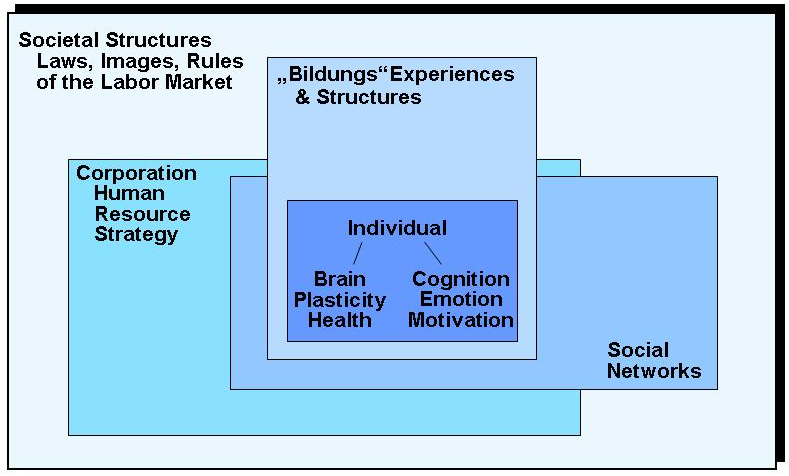
\includegraphics[width=7cm]{deanUrsulaStaudingerIntro.png}
%    \caption{Productive Adult Development at the Jacobs Center: A systemic approach (based on Staudinger, 2006).}\label{fig:deanIntro}
%   \end{center}
%\end{figure}



The developing individual is embedded in different important systems of influence that need to be kept in mind if the process of development is supposed to be productive. These systems are ``Bildungs'' experiences, social networks, the respective corporation with its approach to human resource development and finally the societal framework conditions such as the legal framework of work and education but also the images of aging and ``Bildung'' available in the public. In all these systems, changes have become necessary to accommodate the current transformative processes and enable successful lifelong learning and lifespan development. 


This systemic framework asks for multiple disciplines to be represented at the JCLL, such as Neuroscience and Human Performance, Lifespan Psychology, Health and Personality Psychology, Organizational Behavior (with a focus on learning in the work setting), Media and Communication Sciences (with a focus on images of aging, age-graded medial preferences and media competence), Business Administration, and Lifecourse Sociology and Economics.


The mutual \looseness=-1 dependencies of individual and social change are the focus of JCLL's joint research endeavors. For instance, the contribution of the Jacobs Center to the proposal of a Graduate School of the Social Sciences (BIGSSS) in the context of the Initiative for Excellence of the German Government (DFG / Wissenschaftsrat) lies exactly at the investigation of life-course and lifespan dynamics and their effect on individual and institutional or societal outcomes. Similarly, the interaction between the individual and the organization plays a central role in the first JCLL joint research proposal successful with the BMBF (Federal Ministry for Bildung and Research). In this project - that brings together all JCLL faculty under one common theme - we are interested in the matches and mismatches among employees' attitudes and competencies, the management strategies and work organization of the company as well the organizational climate with regard to the following domains: health promotion, training, images of aging, experience transfer, and adaptive competence. The central assumption is that individual as well as organizational outcomes (e.g., health, productivity) are best understood when taking into consideration the matches and mismatches between all possible combinations (Strategy - Climate, Climate - Employee, Employee - Strategy). Both a linear as well as a typological approach are considered as useful analytical tools. Five companies have agreed to participate. We will pursue a two-step sampling procedure: first we sample work units per company and second we sample individuals within each work unit. In order to keep the assessment protocol to a realistic length not all research domains will be assessed at each company. Rather, always two companies will have one domain in common. Thus, replication of findings across companies becomes possible. The research project, which will start in April 2007, is part of a program initiative by the BMBF revolving around innovative approaches to work security and health protection in the workplace. One of the results of this project will be a diagnostic toolbox for the identification of matches or mismatches in the domains of aging, learning, health, communication and adaptive capacity as well as application rules to be given to companies that want to work with the tool. 


Ursula M. Staudinger\\ 
Bremen, December 2006

\shorttitle{Pure Mathematics}\subsection{Pure Mathematics}
%\input{./MathTheoPhys/Kaimanovich_2005}
%\input{./MathTheoPhys/Litvinov_2005}
%\input{./MathTheoPhys/Penkov_2005}
\begin{bibunit}[plain]
\subsubsection{Number Theory, Arithmetic Geometry, Diophantine Equations}
\index{Stoll, Michael}

\paragraph{Research Team}

Michael Stoll (Professor),
Sebastian Stamminger, (PhD Student, thesis defense in December~2005),
Jan Steffen M\"uller (PhD Student, since September~2006)

\medskip

Most of my research studies the set of
rational points on a curve.  In more elementary terms, I~am looking at the set
of solutions in rational numbers to an equation $F(x, y) = 0$, where
$F$ is a polynomial with integer coefficients.

Such curves are classified according to their genus~$g \ge 0$.
The case $g = 0$ is well understood.
Curves with $g = 1$ either have no rational points at all,  or the set of
rational points forms a finitely generated abelian group;
the problem is then to find generators of this group. Curves
with  $g \ge 2$ have only  finitely many rational points; here the
problem is to find all of them.

There are no general methods that are known to solve these problems.
However, there are methods available that solve these problems in
many concrete cases. Part of my  research tries to extend the range
of cases we can deal with. The other part is about proving general
results.


\paragraph{Highlights}

%500 words about highlights in 2006

In this year, I was mostly continuing work on projects that feature in
previous research reports, with the aim of getting papers ready for
publication. For example, the paper~\cite{Stoll2} on the generalized
Fermat Equation $x^2 + y^3 = z^7$ that I wrote with Bjorn Poonen and
Ed~Schaefer has been finished, submitted and accepted for publication.
Another area of ongoing work is the project on `Explicit $n$-descent
on elliptic curves', which is a joint effort with John Cremona, Tom
Fisher, Cathy O'Neil and Denis Simon. We have finished and submitted
the first two of a series of papers describing our
results~\cite{StollandCFOS1,StollandCFOS2}; the first has just been
accepted by the `Journal f\"ur die reine und angewandte Mathematik'.
Two more papers
are in preparation. Finally, a paper which gives an overview over a
computational experiment that I performed with Nils Bruin has just been
recommended for publication in `Experimental Mathematics',
see~\cite{Stoll4}. Three further papers that describe the details of the
algorithms we used are being written or in preparation. Below,
I will give some more detail on this experiment.

The question we were studying is the following. Given a curve of
genus at least~$2$, defined over the field of rational numbers, is it
possible to decide algorithmically whether it has any rational points?
The most obvious first case to look at is when the genus is~$2$.
In this case, the curve has an equation of the form
\[ y^2 = f_6 x^6 + f_5 x^5 + f_4 x^4 + f_3 x^3 + f_2 x^2 + f_1 x + f_0 \]
where the polynomial on the right hand side has degree $5$ or~$6$ and
does not have multiple roots. For these curves, a number of algorithms
is available and implemented (many of them based on research I have
done). To make the computations feasible and on the other hand not
dependent on random choices, we decided to consider {\em all} such
curves with coefficients $f_0, f_1, \dots, f_6$ from $\{-3,-2,1,0,1,2,3\}$.
Identifying `isomorphic' curves, we had to study about 200,000
different curves.

For each of these curves, we first tried to find a rational point.
This was successful for about 140,000 of them. In a next step, we
checked the curves for `local solubility', which is a necessary
condition for rational points to exist. For example, it may be the
case that the equation does not even have solutions in real numbers.
We were able to prove in this way for about 30,000 curves that they
do not possess rational points. Then we applied a `2-cover descent'
to the remaining about 30,000 curves. This allowed us to test a
stronger necessary condition, at the cost of a much more involved
computation. In this way, all but about 1,500 curves were shown to
have no rational points. Finally, for these remaining curves, we used
another method which needs still more computation, and were able to
prove that none of them has a rational point. For 42 curves, we had
to assume a standard conjecture, otherwise our results are
unconditional. So we could answer the question for all our curves.
This is a very nice result and supports the view that it should
always be possible to decide whether rational points exist or not.


%Pictures are to be included via:
%
\begin{figure}[ht]
  \begin{center}
    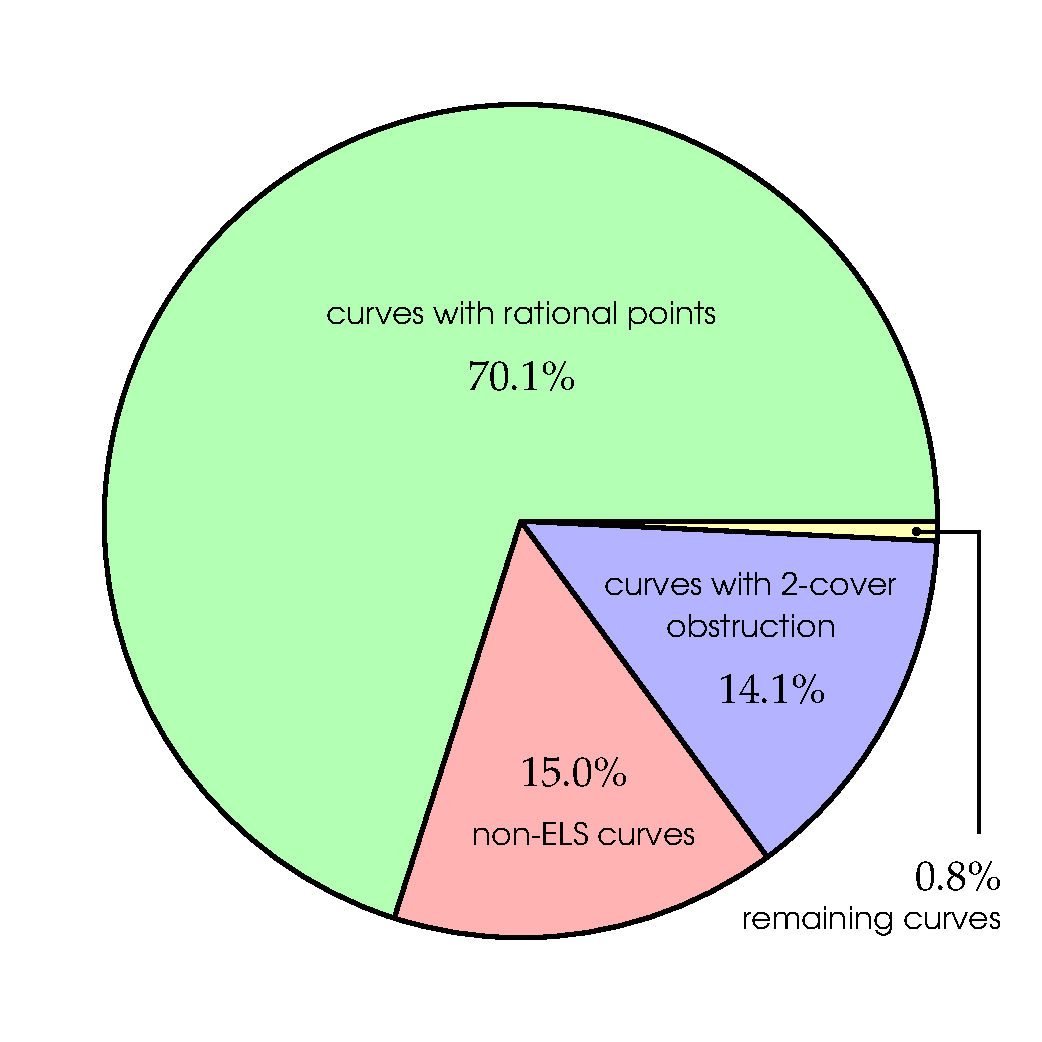
\includegraphics[width=\hsize]{Stoll/profStoll-fig1.pdf}
    \mycaption{Curve statistics (ELS = everywhere locally solvable)}\label{fig:profStoll}
   \end{center}
\end{figure}

\nocite{Stoll1}
\nocite{Stoll3}
\nocite{Stoll5}
\nocite{Stamminger}
\nocite{Stoll6}

\paragraph{Organization}
% list the (research) events you have organized, if any,

\begin{enumerate}
  \item Co-organization of a joint ``Seminar on Algebraic and Arithmetic
        Geometry'' between Universit\"at G\"ottingen, Universit\"at Hannover
        and Jacobs University Bremen
  \item Organization of a training weekend for the German IMO team
        (with Dierk Schleicher and Alexei Belov).
\end{enumerate}

\paragraph{Collaborations}

\begin{enumerate}
  \item {\sl University of California at Berkeley, USA} \\
        Prof.~B.~Poonen \\
        Generalized Fermat Equations, Rational Points on Curves
  \item {\sl University of Santa Clara, California, USA} \\
        Prof.~E.F.~Schaefer \\
        Generalized Fermat Equations
  \item {\sl University of Nottingham, UK} \\
        Prof.~J.E.~Cremona \\
        Descent on Elliptic Curves
  \item {\sl Cambridge, UK} \\
        Dr.~T.A.~Fisher \\
        Descent on Elliptic Curves
  \item {\sl Columbia University, New York, USA} \\
        Asst.~Prof.~C.~O'Neil \\
        Descent on Elliptic Curves
  \item {\sl Universit\'e de Caen, France} \\
        Dr.~D.~Simon \\
        Descent on Elliptic Curves
  \item {\sl Simon Fraser University, Vancouver, Canada} \\
        Asst.~Prof.~N.~Bruin \\
        Rational Points on Curves
  \item {\sl Jacobs University Bremen} \\
        Dr.~S.~Baier \\
        Rational Points on Curves
\end{enumerate}


\paragraph{Grants}
% list the running grants in 2006, if none have been received, please delete this
% subsection.
\begin{enumerate}
  \item Funded by EU, \emph{Galois Theory and Explicit Methods}
        (FP\,6 Research and Training Network, from October~2006;
        I am an external member of the node in Essen)
  \item Funded by DFG, \emph{Arithmetic of K3 Surfaces}

  \item Funded by DFG, \emph{Support for a workshop ``Rational Points on Curves
        and Higher-Dimensional Varieties: Theory  and Explicit Methods''
        at Jacobs University Bremen}, (July 21--28, 2007)
\end{enumerate}


%\paragraph{Awards, Prizes}
% list the grants you have received in 2006, if none have been received, please delete this
% subsection.
%\begin{enumerate}
%\item
%\item
%\end{enumerate}

%Publications should be delivered as a separate file (naming
%convention profxxx.bib. See description by R. Helling. Please make
%sure that all your publications are referred to in the TiX file.
%This can either be in form of a \cite{profxxxkey} or as a
%\nocite{profxxxkey} in the end. A publication which is not
%reffered to on the LaTeX file doesn't produce any output in the
%report.

\putbib[combined]
\end{bibunit}
%\input{./MathTheoPhys/Styrkas_2005}
%\input{./MathTheoPhys/Schleicher_2005}
%\input{./MathTheoPhys/Tikhomirov_2005}
\shorttitle{Applied Mathematics}\subsection{Applied Mathematics}
\begin{bibunit}[plain]
%\svnInfo $Id$
%\svnKeyword $HeadURL$

%\documentclass{article}              
%\usepackage{epsfig}
%\begin{document}

\subsubsection{Visualization and Computer Graphics}
\index{Linsen, Lars}

\paragraph{Research Team}
Lars Linsen (Professor),
Sherin Al-Shbat (PhD Student),
Tetyana Ivanovska (PhD Student),
Tran Van Long (PhD Student),
Paul Rosenthal (PhD Student)

\medskip

Lars Linsen is also involved in  ``Smart Systems''
  (Section \ref{???}). % enter

%The Visualization and Computer Graphics Laboratory (VGCL) led by Prof.~Lars
%Linsen is mainly concerned with topics from scientific and information
%visualization  plus some selected topics from computer graphics and geometric
%modeling.
%
%Visualization is an inherently interdisciplinary field with application in many
%different areas. Scientific visualization deals with the visualization of data
%with spatial interpretation such as computer-generated data from numerical
%simulations (physics, chemistry)  or measured data using scanning or sensoring
%techniques (medicine, life sciences, geosciences). The group's efforts are to
%generate visualization methods that can handle large data sets efficiently,
%filter distinct features automatically or interactively, and display the
%relevant information in a comprehensive and intuitive fashion. The research
%focuses on segmentation and isosurface extraction, hierarchical methods,
%multi-variate data visualization, flow and tensor field visualization, and user
%interaction.
%
%Information visualization deals with the visualization of abstract data  with
%no spatial interpretation such as graph- or network-based data (life sciences,
%social sciences) or multi-dimensional data (databases, ecomomics). The group's
%efforts focus on interactive exploration and analysis tools for such abstract
%data.
%
%In the areas of computer graphics and geometric modeling the group's interest
%lies  in point-based methods, multi-resolution surface representation, and
%curves on surfaces.


\paragraph{Highlights} \strut

{\em A Framework for Real-time Volume Visualization of Streaming Scattered
Data.} Scattered data reconstruction algorithms are often computationally
expensive and difficult to implement.  In order to visualize streaming
scattered data, efficient approaches to scattered data reconstruction are
required.  We have developed a general framework for scattered data
interpolation operating on discrete domains.  The key idea for speeding up the
reconstruction over an underlying grid is a re-factorization of the algorithm. 
The re-factorized version is designed such that it easily maps to graphics
hardware architectures  exploiting their performance and parallelism. Moreover,
it naturally extends to applications for streaming data.  As a proof of
concept, we have implemented inverse-distance-weighted interpolation, natural
neighbor interpolation,  and radial Hermite interpolation using our general
framework. In particular, the natural neighbor interpolation  gained a major
speed-up when exploiting geometrical properties of Sibson's interpolant, which
reduces the $d$-dimensional interpolation problem to rendering $d$-dimensional
spheres of known radii and blending them. We have applied the framework to two
kinds of streaming data: progressive scattered data and real-time sensor data
with moving sensors delivering asynchronous measurements.  To account for the
scattered spatial and temporal distribution of streaming sensor data,  we use a
four-dimensional extension of our framework, which elegantly handles
representation of  time-varying data and leads to reconstructions that are
smooth in both space and time.


\begin{figure}[ht]
  \begin{center}
    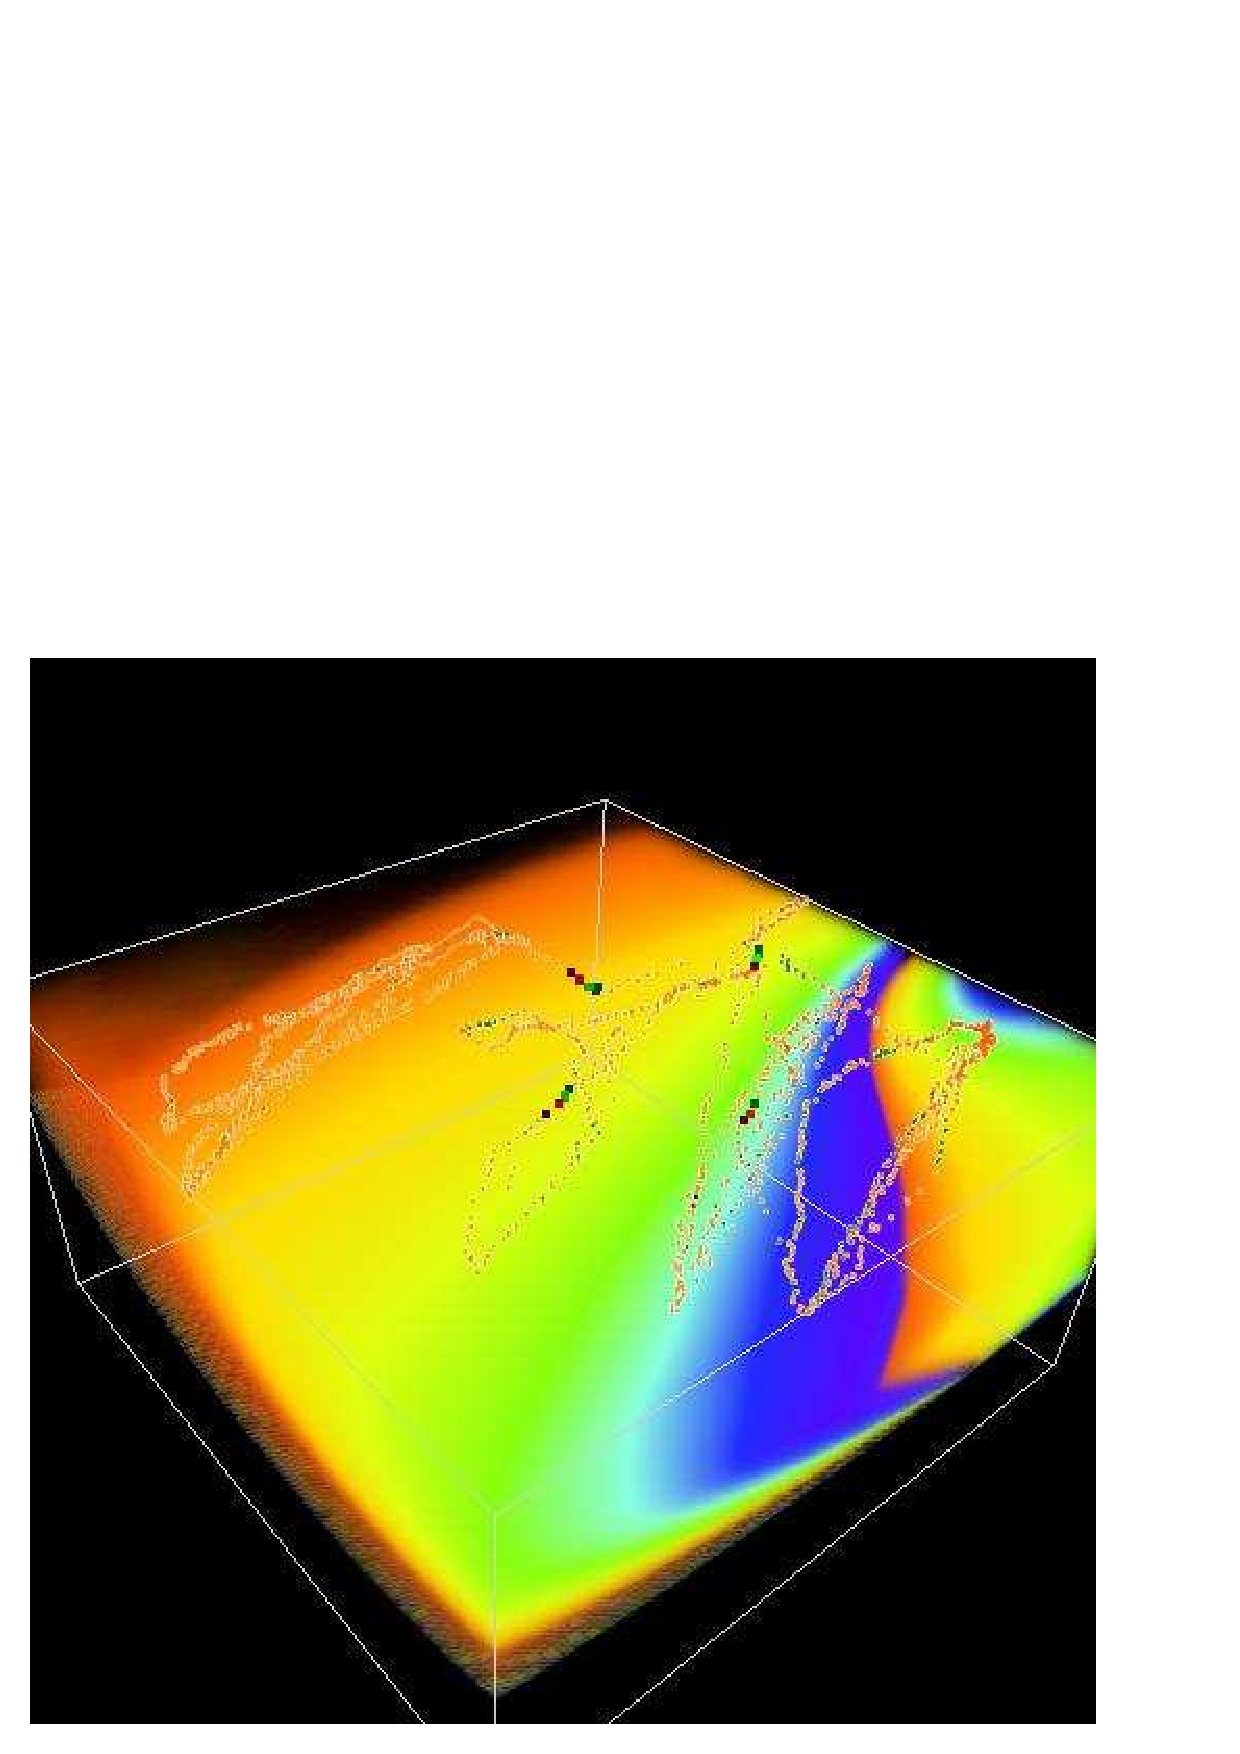
\includegraphics[width=7cm]{MathTheoPhys/Linsen/Linsen_2006_Fig3.pdf}
    \mycaption{Visualization of streaming temperature data in Monterey Bay scattered over time and space. A direct volume rendering of a three-dimensional time-orthogonal hyperplane after reconstruction over a $128 \times 128 \times 64\times 1800$ grid (using natural neighbor interpolation) is shown.}
   \end{center}
\end{figure}

%\end{document}

%%% Local Variables: 
%%% mode: latex
%%% TeX-master: report
%%% End: 

\putbib[combined]
\end{bibunit}
%\input{./MathTheoPhys/Khalili_2005}
%\input{./MathTheoPhys/Oliver_2005}
%\input{./MathTheoPhys/Pfander2_2005}
%\input{./MathTheoPhys/Oswald2_2005}
%\shorttitle{Applied Mathematics)
%\subsection{Theoretical and Computational Physics}
%\input{./MathTheoPhys/Hartmann_2005}
%\input{./MathTheoPhys/Kramer_2005}
%\input{./MathTheoPhys/Ortmanns_2005}
%\input{./MathTheoPhys/Schupp_2005}
%\input{./MathTheoPhys/Brueggen2_2005}
%\input{./MathTheoPhys/Rosswog2_2005}
%\input{./MathTheoPhys/Vogt}
%\shorttitle{Template Test}
%\subsubsection{Research Area }
\index{Name, First Name}

\paragraph{Research Team}
xxx(Professor), xxx (PhD Student)\\

150 words about research in general

\paragraph{Highlights}


500 words about highlights in 2006

Pictures are to be included via:

\begin{figure}[ht]
  \begin{center}
    \includegraphics[width=6cm]{profxxx-figx.jpg}
    \mycaption{ xxx )}\label{fig:profxxx}
   \end{center}
\end{figure}

\paragraph{Organization}
% list the (research) events you have organized, if any,

\begin{enumerate}
\item  xxx
\item  xxx
\end{enumerate}

\paragraph{Collaborations}
\begin{enumerate}
\item {\sl Institution} \\ Partner \\ Research Topic \ Collaboration
\item {\sl Institution} \\ Partner \\ Research Topic \ Collaboration
\end{enumerate}


\paragraph{Grants}
% list the running grants in 2005, if none have been received, please delete this
% subsection.
\begin{enumerate}
\item {Funded by} ``Proposal ��
\item {Funded by} ``Proposal ��
\end{enumerate}


\paragraph{Awards, Prizes}
% list the grants you have received in 2005, if none have been received, please delete this
% subsection.
\begin{enumerate}
\item
\item
\end{enumerate}

Publications should be delivered as a separate file (naming
convention profxxx.bib. See description by R. Helling. Please make
sure that all your publications are referred to in the TiX file.
This can either be in form of a \cite{profxxxkey} or as a
\nocite{profxxxkey} in the end. A publication which is not
reffered to on the LaTeX file doesn't produce any output in the
report.


\shorttitle{References}
\renewcommand{\bibsection}{\paragraph{\refname}\par}
\renewcommand{\refname}{Publications}
\setlength{\bibhang}{0pt}
\bibliographystyle{plainnat}
%\bibliography{ses,report}
%\defaultbibliography{combined}
%\bibliography{combined}
\end {document}
